% Nejprve uvedeme tridu dokumentu s volbami
\documentclass[czech,master,public,dept460,male,oneside,hidelinks]{diploma}
% Dalsi doplnujici baliky maker
\usepackage{float}
\usepackage{amsmath}
\usepackage{amsfonts}
\usepackage{calc}
\usepackage{array}
\usepackage{graphicx}
\usepackage{enumitem}
\usepackage{caption}
\usepackage{siunitx}
\usepackage{subfig}     % makra pro "podobrazky" a "podtabulky"
\usepackage{tikz}       % makra pro kresleni
\usepackage{etoolbox}
\usepackage{multirow}
\usepackage{dirtree}
\usepackage[export]{adjustbox}

\makeatletter   
\let\oldcite\cite
\pretocmd{\listoffigures}{\def\cite{\ignorespaces\@gobble}}{}{}
\apptocmd{\listoffigures}{\let\cite\oldcite}{}{}
\makeatother
\usetikzlibrary{arrows,positioning,plotmarks,decorations.markings,decorations.pathmorphing,backgrounds,fit,positioning,shapes.symbols,chains}
\definecolor{dkgreen}{rgb}{0,0.6,0}
\definecolor{dred}{rgb}{0.545,0,0}
\definecolor{dblue}{rgb}{0,0,0.545}
\definecolor{lgrey}{rgb}{0.99,0.99,0.99}
\definecolor{gray}{rgb}{0.4,0.4,0.4}
\definecolor{darkblue}{rgb}{0.0,0.0,0.6 }
\lstdefinelanguage{cpp}{
      backgroundcolor=\color{lgrey},  
      basicstyle=\footnotesize \ttfamily \color{black} \bfseries,   
      breakatwhitespace=false,       
      breaklines=true,               
      captionpos=b,                   
      commentstyle=\color{dkgreen},   
      deletekeywords={for},          
      escapeinside={\%*}{*)},                  
      frame=single,                  
      language=C++,                
      keywordstyle=\color{purple},  
      morekeywords={vector, Size ,string, Rect,HOGDescriptor,size_t,Mat,}, 
      identifierstyle=\color{black},
      stringstyle=\color{blue},      
      numbers=left,                 
      numbersep=5pt,                  
      numberstyle=\tiny\color{black}, 
      rulecolor=\color{black},        
      showspaces=false,               
      showstringspaces=false,        
      showtabs=false,                
      stepnumber=1,                   
      tabsize=5,                     
      title=\lstname,                 
    }



% Zadame pozadovane vstupy pro generovani titulnich stran.
\ThesisAuthor{Jakub Ševčík}

\CzechThesisTitle{Detekce chodců na embedded systémech}

\EnglishThesisTitle{Pedestrian Detection on Embedded Systems}

\SubmissionDate{30. dubna 2018}

% Pokud nechceme nikomu dekovat makro zapoznamkujeme.
\Thanks{Rád bych na tomto místě poděkoval všem, kteří mi s~prací pomohli, protože bez nich by tato práce nevznikla.}

% Zadame cestu a jmeno souboru ci nekolika souboru s digitalizovanou podobou zadani prace.
% Pokud toto makro zapoznamkujeme sazi se stranka s upozornenim.
\ThesisAssignmentImagePath{figures/assignment}

% Zadame soubor s digitalizovanou podobou prohlaseni autora zaverecne prace.
% Pokud toto makro zapoznamkujeme sazi se cisty text prohlaseni.
%\AuthorDeclarationImageFile{figures/AuthorDeclaration.jpg}

%\ThesisAccessRestriction{Zde vložte text dohodnutého omezení přístupu k Vaší práci, chránící například firemní know-how. Zde vložte text dohodnutého omezení přístupu k Vaší práce, chránící například firemní know-how. A zavazujete se, že:
%\begin{enumerate}
%\item podle \textsection{} 5 o práci nikomu neřeknete,
%\item po obhajobě na ni zapomenete a
%\item budete popírat její existenci.
%\end{enumerate}
%A ještě jeden důležitý odstavec. A ještě jeden důležitý odstavec.
%A ještě jeden důležitý odstavec. A ještě jeden důležitý odstavec.
%A ještě jeden důležitý odstavec. A ještě jeden důležitý odstavec.
%Konec textu dohodnutého omezení přístupu k Vaší práci.}

% Zadame soubor s digitalizovanou podobou souhlasu spolupracujici prav. nebo fyz. osoby.
% Pokud toto makro zapoznamkujeme sazi se cisty text souhlasu.
%\CooperatingPersonsDeclarationImageFile{Figures/CoopPersonDeclaration.jpg}

\CzechAbstract{Cílem práce je prozkoumat dosavadní techniky rozpoznávání chodců v~obrazech.  Primárním cílem práce je otestovat a~pokusit se optimalizovat tyto rozpoznávácí algoritmy na vybraných embedded zařízeních. K~rozpoznávání byly použity knihovny OpenCV a~Dlib. Použité algoritmy jsou popsány v~textu. Součástí práce je také srovnání úspěšnosti a~rychlosti jednotlivých detektorů. }

\CzechKeywords{detekce chodců, embbeded systémy, optimalizace}

\EnglishAbstract{The goal of work is to explore the existing techniques of pedestrian detection in scenes. The primary objective of the thesis is to test and attempt to optimize these detection algorithms on selected embedded devices. For detection were used the OpenCV and Dlib libraries. The algorithms used are described in the text. Part of the thesis is also a~comparison of the successful and speed of individual detectors.}

\EnglishKeywords{Pedestrian Detection, Embedded Systems, optimalization}

\AddAcronym{ALG}{Algoritmus}
\AddAcronym{API}{Application Programming Interface - rozhraní pro programování aplikací}
\AddAcronym{ARM}{Advanced RISC Machine - architektura počítačů s~nízkou elektrickou spotřebou energie}
\AddAcronym{C++}{Programovací jazyk C Plus Plus}
\AddAcronym{Dlib}{Otevřená cross-platform knihovna pro zpracování obrazu a~strojového učení}
\AddAcronym{FPS}{Frames per second - Počet snímků za sekundu}
\AddAcronym{IoT}{Internet of Things - Internet věcí}
\AddAcronym{MMX}{Multi Media Extension, multimediální technologie vytvořené firmou Intel}
\AddAcronym{NEON}{Pokročilé rozšíření architektury SIMD pro procesory ARM Cortex-A a~Cortex-R52 }
\AddAcronym{OpenCV}{Otevřená knihovna pro zpracování obrazu a~strojového učení}
\AddAcronym{RGB}{Red Green Blue - barevný prostor složený ze tří barevných kanálů}
\AddAcronym{SIMD}{Single Instruction Multiple Data - typ počítačové architektury}
\AddAcronym{SSE}{Streaming SIMD Extensions je instrukční sada typu SIMD}
\AddAcronym{SVM}{Support vector machines}
\AddAcronym{XML}{Extensible Markup Language}
\AddAcronym{YML}{YAML Ain't Markup Language}



% Zacatek dokumentu
\begin{document}
% Nechame vysazet titulni strany.
\MakeTitlePages

% Pokud mame v zaverecne praci vypisy kodu, jinak odstranit.    
\lstlistoflistings
\section{Úvod}
Detekce chodců je velmi náročný úkol, který v~posledních letech přitahuje velkou pozornost. 
Aplikace tohoto typu mohou mít široké uplatnění jak v~osobním, tak v~industriálním využití. Může se jednat o~bezpečnostní prvky, například na letištích, kde program může sledovat pohyb daného chodce a~vyhodnocovat tak jeho chování, jakým je kamera průmyslového vozidla, kde řidič může přehlédnout chodce v~blízkosti vozidla, a~předejít tak neštěstí, kdy program může zamezit pohybu vozidla. Dalšími příklady mohou být detekce chodců na přechodech pro chodce, v~továrnách, kde se může pomocí rozšíření algoritmu o~rozpoznání obrazu vyhodnocovat chování a~docházka zaměstnanců. 

Nutno podotknout, že detekce chodců v~obrazech není pro lidi tak obtížným ůkolem a~dokážou bez větší námahy rozpoznat všechny osoby v~obraze. Pro stroje je naopak tento úkol velkou výzvou. Chodci v~obrazech mohou mít různý tvar těla, barvu kůže, jiný postoj, také různý počet vrstev a~barev oblečení na sobě. Mohou být také z~části zakrytí nějakým objektem v~obraze, který nepodléhá samotné detekci, což může způsobit záporné vyhodnocení. Také zde má velký vliv vzdálenost osoby od kamery, kdy se pro strojovou doménu může stát chodec nedetekovatelný. 

Velkou zásluhu na strojovém detekování chodců má Navneet Dalal a~Bill Triggs, kde ve své práci \cite{hog:dalal} pomocí metodiky histogramu orientovaných gradientů úspěšně detekují chodce v~obrazech. Tato práce se z~větší části inspiruje tímto dokumentem a~rozšiřuje jej o~substrakci pozadí, která má za úkol urychlit a~zlepšit samotnou detekci chodců v~obrazech. Principem tohoto algoritmu je spustit detekci pouze v~oblastech obrazu, který není statický, a~kdy se tedy nemusí jednat o~chodce. Ovšem tento typ algoritmu lze použít pouze na videosnímcích, které jsou pořízené ze statické kamery.

Hlavním cílem této práce bylo optimalizovat a~otestovat detektor chodců pro počítače s~architekturou ARM a~využít tak jejich značný výkon. 
Experimenty této práce se zaměří jak na trénování a~testování klasifikátoru s~různými parametry, tak na detekci chodců na samostatných snímcích, ale také i~ve videosekvencích, které budou detailně zaznamenány a~vyhodnoceny. 
V~druhé kapitole budou představeny hlavní výzvy a~problémy detekce chodců v~obrazech.
Jedna z~kapitol se bude věnovat metodikám pro detekci chodců a~využitých knihoven pro zpracování obrazu v~této práci.
V~dalších kapitolách bude popsána implementace programu, popis jeho funkcí, kterými tato aplikace disponuje. Také zde budou uvedena a~popsána zařízení, na kterém byl otestován. V~neposlední řádě experimenty a~jejich dosažené výsledky.
\section{Výzvy a problémy detekce chodců}
Detekce chodců je nezbytným a významným úkolem v jakémkoliv inteligentním kamerovém systému, protože poskytuje základní informace pro sémantické porozumění videosekvence. Tohle rozšíření má zásadní prospěch v automobilovém průmyslu z důvodu možného zlepšení bezpečnostních systémů. Mnoho výrobců aut již tuto funkcionalitu nabízejí ve svých vozech jako ``Pokročilé systémy asistence řidiče'' (ADAS) od roku 2017.

Bohužel ne vždy detektor může rozpoznat chodce v obraze, a to může být ovlivněno několika faktory. Takovými faktory můžou být:

\subsection{Tvar těla (póza, držení těla)}
Chodec v obraze může mít neobvyklý postoj těla, chůzi nebo různé proporce a stavbu těla. Lidské tělo může být z části zakryto nějakým objektem ze scény nebo se nemusí vyskytovat celé v záběru snímku. Takový člověk může být snadno identifikovatelný pro lidské oko, ale pro stroje může představovat velkou výzvu. 

\subsection{Barva kůže}
Barva kůže může také představovat problém pro rozpoznání chodce. Na světě existují různé druhy pigmentace kůže a jejich odstíny se pohybují v rozmezí od nejtmavší hnědé až po nejsvětlejší odstíny. Příklady barev kůže ilustruje obrázek \ref{colorskin}.

\begin{figure}[H]
\centering
\includegraphics[width=15cm]{figures/colorskin}
\caption{Příklady druhů pigmentace kůže\cite{skincolor:obr}}
\label{colorskin}
\end{figure}

\subsection{Vnější podněty}
Problém pro identifikování chodce v obraze může také představovat druh osvětlení scény, případně střídání dne a noci pro venkovní kamerové systémy. Také zde hraje důležitou roli nastavení a vlastnosti dané kamery. 

\subsection{Oblečení a různé doplňky}
Do této kategorie mohou spadat například zimní oblečení, které můžou zvětšit objem, či tvar těla, nebo různě rozměrné pokrývky hlavy. Chodec také může nést nějaké předměty, které mohou zakrývat nebo splývat s jeho části těla. Tyto aspekty mohou také ovlivnit detekci.

\subsection{Pozice v obraze}
Osoby se mohou nacházet libovolně kdekoliv v obraze, mohou jít čelem k ohnisku kamery nebo mohou být zachyceni pouze z boku. Například kamera umístěná ve výšce pouličního osvětlení v nějakém předem určeném úhlu, snímá obraz z určité perspektivy. Tato kamera pak zajištuje velikou škálu chodců v různém měřítku. Pro stroj tohle může být ovšem problematické. Osoby ve větším měřítku můžou být snadno detekovatelné, ovšem chodci, kteří jsou hodně vzdálení v obraze nikoliv. V tomto případě také závisí na nastavení daného detektoru za cenu pomalejší a méně přesnější detekce. 

\subsection{Pozadí (prostřední scény)}
Chodci se mohou vyskytovat v komplexním prostředí. Opět pro lidské oko může být člověk snadno identifikovatelný a pro doménu strojů se může tato situace jevit jako neproveditelná. Osoba v obraze může totiž dokonale splynout s prostředním, které se za ním nachází.  

Příklad výše zmíněných výzev a problémů detekce najdeme v obrázku \ref{pedestrians}, který je umístěn níže. V tomto ilustrativním obrázku najdeme osoby s různě barevným oblečením různého tvaru. Chodci se zde nacházejí v různém úhlu k ohnisku kamery. 

\begin{figure}[H]
\centering
\includegraphics[width=15cm]{figures/pedestrians}
\caption{Ukázka chodců v obraze}
\label{pedestrians}
\end{figure}
\section{Metody detekce chodců}
V~této kapitole budou popsány nejpoužívanější a~nejznámější detekční metodiky. Všechny implementace těchto metodik jsou dostupné minimálně v~jedné knihovně použité v~této práci. Prvně budou uvedeny metody založené na příznacích, jmenovitě Histogram orientovaných gradientů, Haar vlnky, Lokální binární vzory a~některé jejich kombinace. Také jsou zde uvedeny klasifikátory Support vector machine a~AdaBoost. V poslední části této sekce se budu věnovat neuronovým sítím. 

\subsection{Metody založené na příznacích}
Navzdory všem výzvám a~problémům detekce chodců zůstává tato oblast výzkumu stále aktivní a~byla navržena řada přístupových technik.
%@TODO
\subsubsection*{Histogram orientovaných gradientů}
Tato metoda vznikla v~roce 2005 za účelem detekování chodců v~obrazech a~je založena na histogramech orientovaných gradientů (\textit{HOG - Histogram of Oriented Gradients}). Autoři této metodiky jsou N. Dalal a~B. Triggs \cite{hog:dalal}. Základní myšlenka spočívá v~tom, že okolní vzhled a~tvar objektu může být často charakterizován distribucí intenzity gradientů nebo směry hran, aniž by byly přesně známy odpovídající gradientové nebo hranové polohy.  

Před samotným výpočtem příznaků by mělo dojít k~zajištění normalizaci barev a~gamy, v~případě černobílých obrázků k~normalizaci kontrastu. Tento krok může být vynechán, jak zdůrazňují autoři Dalal a~Triggs. Normalizace deskriptorů dosahují stejného výsledku, a~tedy předběžné zpracování obrázku má malý vliv na výkon. Místo toho je prvním krokem výpočet gradientních hodnot. Nejběžnější metodou je aplikování jednodimenzionální derivační masky v~jednom nebo obou směrech, jak horizontálním tak vertikálním. Autoři také experimentovali s~komplexnějšími maskami, jako je například $3x3$ Sobelova maska, nebo diagonální masky, avšak tyto masky se prokázaly jako méně účinné. Stejně tak neúčinné bylo použití jakéhokoliv vyhlazení obrazu před aplikací derivační masky. Autoři této metody přišli na to, že nejlepší kombinací je použití konvolucí Gaussovského filtrování $\sigma = 0$ na obraze $I$ s~maskou $[-1, 0, 1]$, $[-1,0,1]^\top$:
\begin{equation*}
\centering
 \label{eq:hogMask}
 \begin{aligned}
I_x = I~* [-1, 0, 1], \\
I_y = I~* [-1, 0, 1]^\top
 \end{aligned}
\end{equation*}
kde:
\begin{itemize}[label=]
  \item $*$: konvoluce,
  \item $I$: obraz.
\end{itemize}

V~druhém kroku dochází k~vytvoření histogramu v~každé buňce, která je standardně tvořena $8x8$ pixely. Každý pixel v~buňce má svou váhu, kterou se podílí na vytvoření orientovaného histogramu, založeného na hodnotách nalezených ve výpočtu gradientu. Hodnoty buněk jsou rovnoměrně rozloženy do histogramu o~9 kanálech (binech) po \ang{20}. Pokud směr gradientu buňky vyjde na pomezí dvou binů, přičte se její magnituda do obou těchto binů.
Tyto buňky spojíme do větších propojených bloků z~důvodu normalizace osvětlení a~kontrastu. Pro chodce se používá L2--norm normalizace, dle vztahu \eqref{eq:normHog}. Tyto bloky se typicky překrývají, což znamená, že každá buňka přispívá více než jednou do finálního deskriptoru. Proces zpracování deskriptoru je ilustrován na obrázku \ref{hog_chain}. Existují dvě varianty spojení bloků, tzv. obdélníkové bloky (R--HOG) a~kruhové bloky (C--HOG), tyto bloky jsou na obrázku \ref{variants_block}.  
\begin{equation}
\centering
 \label{eq:normHog}
 \begin{aligned}
L2-norm&: \qquad  f =& \frac{v}{\sqrt{\lVert v~\lVert_2^2 + e^2}} \\
L1-sqrt&: \qquad  f =& \sqrt{\frac{v}{\lVert v~\lVert_1 + e}}
 \end{aligned}
\end{equation}
Nechť $v$ je nenormalizovaný vektor obsahující všechny histogramy v~daném bloku, $\lVert v \lVert_k$ je jeho k--norm pro $k = 1,2$, a~$e$ je malá konstanta.
 \begin{figure}[H]
\centering
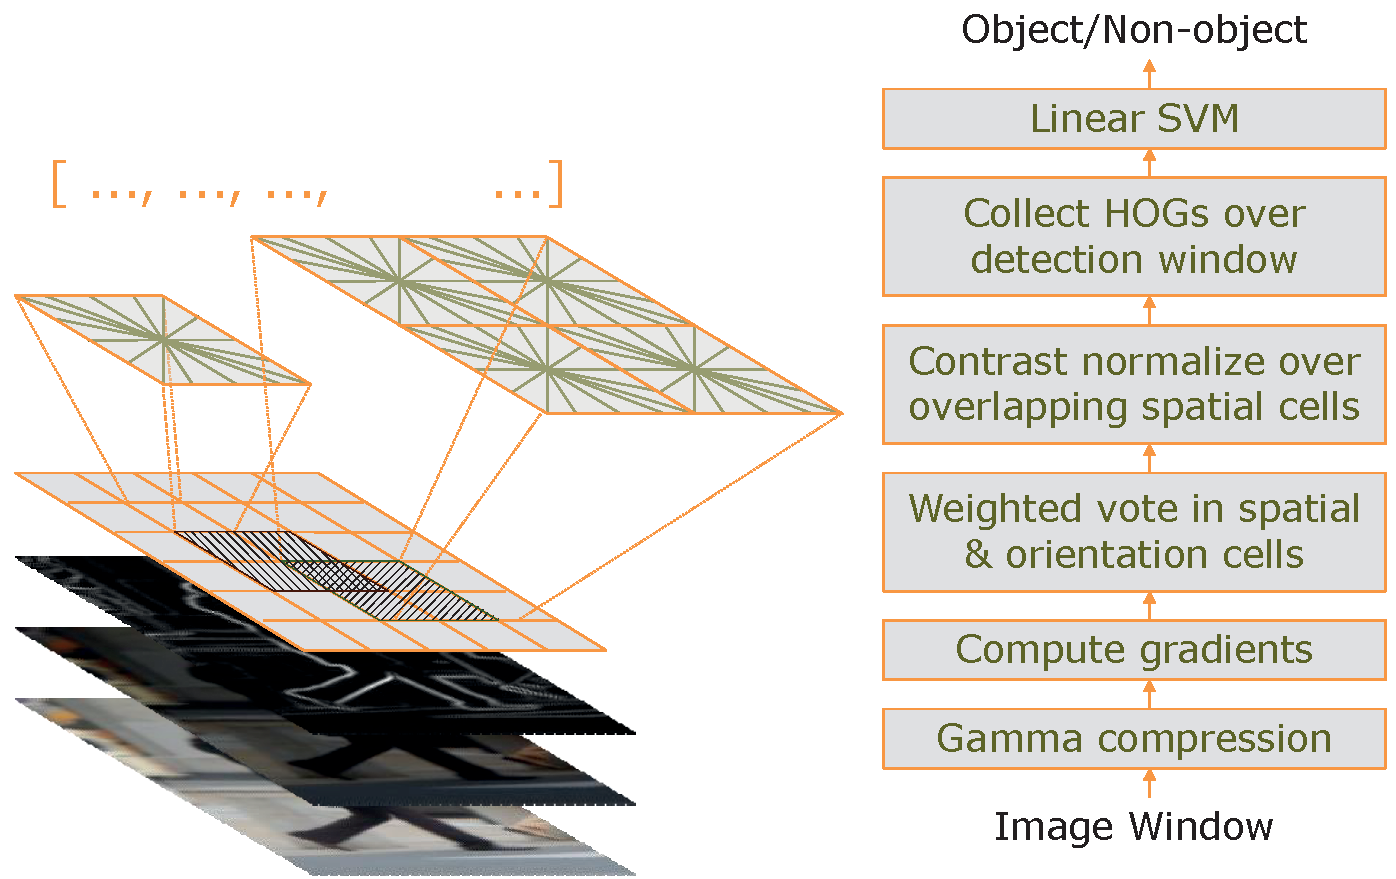
\includegraphics[width=16cm]{figures/hog_pipeline}
\caption{Procesní řetezec výpočtu deskriptoru \cite{hog:dalal}}
\label{hog_chain}
\end{figure}

\textbf{C--HOG} (Kruhové HOG bloky) - lze nalézt ve dvou variantách: \textit{s~jedinou, centrální buňkou} a~\textit{úhlově rozdělenou centrální buňkou}. Dají se popsat čtyřmi parametry: počtem úhlů a~radiálních kanálů (binů), poloměrem centrálního binu a~faktorem roztažení pro poloměr dalších radiálních binů.  Tyto bloky se podobají deskriptorům kontextu tvarů (shape context descriptors \cite{shapeContext}), ale C--HOG jsou buňky s~několika orientovanými kanály, zatímco shape context využívají přítomnost jediné hrany.

\textbf{R--HOG} (Obdélníkové HOG bloky) - tyto bloky jsou v~praxi nejčastěji používané a~reprezentují se třemi parametry: \textit{počet buněk na blok}, \textit{počet pixelů na buňku} a~\textit{počet binů (kanálů) na jeden histogram}. Bloky se zdají podobné deskriptorům transformací příznaků invariantní vůči měřítku (scale--invariant feature transform SIFT \cite{siftPaper}), avšak liší se výpočtem bloků. R--HOG bloky jsou vypočteny v~hustých mřížkách v~libovolném měřítku bez zarovnání orientace, zatímco SIFT deskriptory obvykle v~mřížkách řídkých, obrazové body invariantní vůči měřítku jsou otočeny, aby přiléhaly orientaci. R--HOG bloky se také používají pro kódování informací. 
\begin{figure}[H]
  \centering
  \includegraphics[width=14cm]{figures/hog_variants.pdf}
  \caption{Varianty geometrie spojení bloků \cite{hog:dalal}}
  \label{variants_block}
\end{figure}
V~knihovně OpenCV existuje funkce \uv{detectMultiScale}, která pomocí \textbf{posuvného okénka} (sliding window) projde celý obraz a~v~každém takovém okně se vypočítávají příznaky. Jeho velikost můžeme definovat pomocí parametru, standardní velikost je $64x128$ pixelů a~následující popis a~výpočty budou odpovídat této velikosti posuvného okna.  

V~tomto okně se obrázek rozdělí na $8x8$ bloků a~v~každém bloku se vypočte histogram magnitud, které se podle směru hrany rozdělují do 9~binů. Vyjde nám vektor o~velikosti 9 a~tyto vektory spojíme do bloků o~velikosti $16x16$ a~normalizujeme je na velikost 1, aby byly nezávislé na osvětlení, dostaneme tedy vektor o~velikosti 36. Na konci tohoto procesu všechny vektory spojíme a~získáme vektor všech příznaků z~konkrétního vzorku nebo z~oblasti zájmu posuvného okénka. Obrázek \ref{fig:hogCalc} zobrazuje vstup vzorku pro vypočítání jeho příznaků neboli histogramu orientovaných hran. Kde nejprve obrázek převedeme do stupně šedi, provedeme normalizaci kontrastu a~gamy a~následně vypočítáme jeho vektor příznaků.
Ukázka dělení obrazového okna je na obrázku \ref{hog_cells}.

 \begin{figure}[H]
\centering
\includegraphics[width=3.6cm]{figures/hog_cells}
\caption{Rozdělení obrazu do $8\times8$ buněk \cite{hog:obr}}
\label{hog_cells}
\end{figure}

\begin{figure}[H]
\centering
\begin{minipage}{.3\textwidth}
  \centering
  \includegraphics[width=.5\linewidth]{figures/hog_input}
  \caption*{Vstupní obrázek}
  \label{fig:hog_input}
\end{minipage}%
\begin{minipage}{.3\textwidth}
  \centering
  \includegraphics[width=.5\linewidth]{figures/hog_histogram_before}
  \caption*{Normalizace kontrastu}
  \label{fig:hog_contrast}
\end{minipage}%
\begin{minipage}{.3\textwidth}
  \centering
  \includegraphics[width=.5\linewidth]{figures/features}
  \caption*{Výpočet příznaků}
  \label{fig:hog_features}
\end{minipage}
\caption{Normalizace a~výpočet příznaků pro obrázek}
\label{fig:hogCalc}
\end{figure}

\subsubsection*{Haarovy příznaky}
Na tomto přístupu je založen objektový detektor Viola--Jones (\textit{Viola--Jones object detector framework}) \cite{violajones}, který poskytuje v~reálném čase spolehlivou a~konkurenceschopnou detekci objektů. Tento systém byl navržen v~roce 2001, a~i~když může být vycvičen pro detekci různých objektových tříd, byl primárně použit především pro detekci obličeje. Detektor pracuje s~obrazy ve stupních šedi a~skládá se ze tří částí. Z~integrálního obrazu, Haarových příznaků a~AdaBoost\cite{adaboost} algoritmu. Tento algoritmus bude popsán v sekci o klasifikátorech. 
Integrální obraz je takový obraz (obrázek \ref{fig:integralimage}), kde každý bod $x$ představuje součet hodnot předchozích pixelů doleva a~nahoru. Spodní pravý bod obsahuje součet všech pixelů v~obraze.
Zápis integrálního obrazu je:
\begin{equation*}
\label{integralimage}
 I(x, y) = \sum_{\substack{x' \leq x \\ y' \leq y}}{} i(x', y'),
\end{equation*}
kde $i(x', y')$ je hodnota pixelu na pozici $(x, y)$.
\begin{figure}[H]
\centering
\begin{minipage}{.4\textwidth}
  \centering
  \includegraphics[width=.5\linewidth]{figures/ii_input}
  \caption*{Vstupní obraz}
  \label{fig:ii_input}
\end{minipage}%
\begin{minipage}{.4\textwidth}
  \centering
  \includegraphics[width=.5\linewidth]{figures/ii_output}
  \caption*{Integrální obraz}
  \label{fig:ii_output}
\end{minipage}
\caption{Převod obrazu na integrální obraz}
\label{fig:integralimage}
\end{figure}

Princip využítí Haarových příznak v~obrazech je založen na pozorování, že lidská těla a~obličeje mají některé podobné rysy. Právě tyto rysy mohou být porovnány pomocí Haarových příznaků. Jedná se například o~tyto rysy:
\begin{itemize}
  \item{Oční oblast je tmavší než oblast nosního mostu,}
  \item{hlava člověka je tmavší než její okolí,}
  \item{oblast mezi dolními končetinami je světlejší než samotné nohy.}
\end{itemize}
Sada Haarových vlnek je na obrázku \ref{fig:basichaarfeatures}, jedná se pouze o~základní sadu příznaků.
\begin{figure}[H]
\centering
\includegraphics[width=.7\linewidth]{figures/haar_features}
\caption{Základní sada Haarových příznaků}
\label{fig:basichaarfeatures}
\end{figure}

Pro identifikaci lidských postav se používá rozšířená sada vlnek, tzv. Haar--like příznaky. Autoři v~publikaci \cite{haar:like} představili novou sadu Haar vlnek pro detekci lidí v~obrazech. Klasifikační systém založený na těchto příznacích dosahuje nížší false positive detekce než původní Haar--like příznaky.  Na obrázku \ref{fig:haarlike} je příklad detekce pomocí Haar--like vlnek ze zmíněné publikace. Hodnota příznaku je rozdíl mezi sumou hodnot pixelů v~bílé a~černé oblastí Haarových vlnek.
\begin{figure}[H]
\centering
\includegraphics[width=.8\linewidth]{figures/haar-like}
\caption{Použití Haar--like příznaků na chodcích \cite{haar:like}}
\label{fig:haarlike}
\end{figure}

\subsubsection*{Lokální binární vzor}
Metoda LBP (Local Binary Pattern) byla navržena pro klasifikaci textur v~obrazech v~roce 1990 \cite{lbp:texture}. Poprvé však byla popsána až v~roce 1994 \cite{lbp:first}. Hlavní myšlenkou LBP je, že struktury obrazu mohou být efektivně zakódovány porovnáním hodnot jednotlivých pixelů a~jejich okolí. Tato metoda je odolná vůči jasovým změnám obrazu.

Prvním krokem této metody je převod obrazu do stupně šedi a~jeho rozdělení do buněk. Okolní hodnoty pixelů jsou porovnávány se středovým pixelem, pokud je jejich hodnota rovna nebo větší zapíše se na tuto pozici jednička v~opačném případě nula. Tyto hodnoty seřadíme buď podle hodinových ručiček nebo naopak a~získáme osmimístné binární číslo, které převedeme do dekadické soustavy. V~následujícím kroku z~čísel, které jsme získali kombinací pixelů v~buňkách, vypočítáme histogram. V~posledním kroku zřetězíme všechny histogramy buněk a~získáme vektor příznaků pro celý obraz. Jedná se o~256--dimenzionální vektor příznaků. 
Matematicky lze LPB vyjádřit jako:
\begin{equation*}
LBP_{P,R} = \sum_{p=0}{P-1} s(g_p - g_c)2^P, \\
s(x) =
  \begin{cases} 
   1 & \text{pro } x \geq 0, \\
   0       & \text{pro } x < 0,
  \end{cases}
\end{equation*}
kde: $P$ je počet bodů v~okolí, $R$ vyjadřuje vzdálenost bodů od středového pixelu, $g_c$ je středový pixel, $g_p$ je aktuální pixel. 

Následující příklad se vztahuje k~obrázku \ref{fig:lbpsum}. Po porovnání pixelů se středovým pixelem jsme získali vzor $11110001$. Tento vzor převedeme do dekadické soustavy a~sečteme, $ 1+16+32+64+128 = \textbf{241}$. Získali jsme hodnotu této buňky do vektoru příznaků.

\begin{figure}[H]
\centering
\begin{minipage}[b]{.3\textwidth}
  \centering
  \includegraphics[width=.5\linewidth]{figures/lbp_img}
  \caption*{Vstupní buňka}
  \label{fig:lpbimg}
\end{minipage}%
\begin{minipage}[b]{.3\textwidth}
  \centering
  \includegraphics[width=.5\linewidth]{figures/lbp_thresh}
  \caption*{Prahové hodnoty}
  \label{fig:lbpthresh}
\end{minipage}
\begin{minipage}[b]{.3\textwidth}
  \centering
  \includegraphics[width=.5\linewidth]{figures/lbp_weights}
  \caption*{Pixely ohodnoceny váhou}
  \label{fig:lbpweights}
\end{minipage}
\caption{Výpočet příznaku}
\label{fig:lbpsum}
\end{figure}

Výhoda této metody je její rychlý a~snadný výpočet a~odolnost vůči různým osvětlením. Na druhou stranu je těžší na trénování, protože výsledné dekadické číslo může mít obrovské množství možností (podle parametru $P$). K~omezení můžeme využít uniformní vzory (obrázek \ref{fig:lbpvzory}). Pro parametr $P=8$, získáme 59 vzorů. 

\begin{figure}[H]
\centering
\begin{minipage}[b]{.18\textwidth}
  \centering
  \includegraphics[width=.9\linewidth]{figures/lbp_spot}
  \caption*{Spot}
\end{minipage}
\begin{minipage}[b]{.18\textwidth}
  \centering
  \includegraphics[width=.9\linewidth]{figures/lbp_spot_flat}
  \caption*{Spot/Flat}
\end{minipage}
\begin{minipage}[b]{.18\textwidth}
  \centering
  \includegraphics[width=.9\linewidth]{figures/lbp_line}
  \caption*{Line}
\end{minipage}
\begin{minipage}[b]{.18\textwidth}
  \centering
  \includegraphics[width=.9\linewidth]{figures/lbp_corner}
  \caption*{Corner}
\end{minipage}
\begin{minipage}[b]{.18\textwidth}
  \centering
  \includegraphics[width=.9\linewidth]{figures/lbp_edge}
  \caption*{Edge}
\end{minipage}
\caption{Lokální okolí LBP metody \cite{lbp:orig}}
\label{fig:lbpvzory}
\end{figure}

\subsubsection*{HOG + LBP}
Kombinace techniky histogramů orientovaných hran a~lokálního binárního vzoru tvoří nový způsob, jak vytvořit sadu příznaků. Ta je schopna manipulovat i~s~částečnou okluzí. Jak autoři publikace \cite{hoglpb} zmiňují, jeden detektor slouží ke globálnímu skenování obrazu a~druhý detektor pro konkrétní oblasti. Oba jsou naučeni z~trénovacích dat lineárního klasifikátoru SVM. Pro každé nejednoznačné skenovací okénko se vytvoří pravděpodobnosti okluze dle odezvy každého bloku HOG příznaku na globální detektor (obrázek \ref{fig:hoglbp}). Tyto pravděpodobnosti okluze se dále segmentují metodou Mean shift \cite{meanshift1} \cite{meanshift2}. Segmentovaná část okna s~větší negativní odpovědí je označena jako okludovaná část. Pokud je indikována okluze s~vysokou pravděpodobností v~nějakém skenovacím okénku, část detektorů je aplikována na oblasti bez okluze k~dosažení konečné klasifikace aktuálního skenovacího okna. 

\begin{figure}[H]
\centering
\includegraphics[width=.6\linewidth]{figures/hoglbp_obr}
\caption{ První řádek ilustruje nejednoznačné výstřižky ze skenovacího okénka. Druhý řádek zobrazuje segmentové pravděpodobnostní okluze odpovající k~obrazům z~prvního řádku.\cite{hoglpb}}
\label{fig:hoglbp}
\end{figure}

\subsubsection*{HOG + LUV}
Tato metoda využívá Histogram orientovaných gradientů a~LUV kanály obrazů pro extrakci příznaků. Kanály RGB vzorku se převedou na kanály LUV. Z~každého kanálu se samostatně vypočtou příznaky, tento převod ilustruje obrázek \ref{fig:luv}. Tyto příznaky můžeme spojit do jednoho vektoru příznaků nebo využít jen některé z~nich. Kanál $L$ je složka luminiscence (jas) a~kanály $UV$ značí sytost barev. 

\begin{figure}[H]
\centering
\begin{minipage}[b]{.3\textwidth}
  \centering
  \includegraphics[width=.8\linewidth]{figures/rgb_luv}
  \caption*{RGB kanály}
\end{minipage}%
\begin{minipage}[b]{.3\textwidth}
  \centering
  \includegraphics[width=.8\linewidth]{figures/luma}
  \caption*{Luminiscence  (L)}
\end{minipage}
\begin{minipage}[b]{.3\textwidth}
  \centering
  \includegraphics[width=.8\linewidth]{figures/uv_chroma}
  \caption*{Sytost barev (UV)}
\end{minipage}
\caption{Rozdíl mezi RGB a~LUV kanály. Obrázek je obsažen v~trénovací sadě Das\cite{sudipdas}.}
\label{fig:luv}
\end{figure}

\subsection{Detekce chodců a~detekce pohybu} % @TODO 
Další možností detekce chodců v~obraze je substrakce pozadí, díky které můžeme extrahovat dynamické části v~obraze. Použitím této metodiky kombinované například s~přístupem založeným na příznacích, můžeme získat rychlý a~optimální detektor.

\subsubsection*{Mixtura Gaussiánů}
Mixtura Gaussiánů (\textit{MOG - Gaussian mixture model background subtraction}) \cite{mog:zivkovic} je metoda substrakce pozadí. Je to široce používaná technika pro generování masky popředí pomocí statických kamer. Jak už jde poznat z~názvu, algoritmus vypočítává masku popředí odečtením referenčního modelu od aktuálního snímku. Referenční model většinou bývá první snímek videosekvence. Dále se na masku aplikuje prahování, čím se vyfiltruje přebytečný šum v~masce, tento postup zobrazuje obrázek \ref{mog_scheme}.

Skládá se ze dvou hlavních kroků:
 \begin{enumerate}
    \item{Inicializace pozadí,}
    \item{aktualizace pozadí.}
 \end{enumerate}
 V~prvním kroku je vypočítán model pozadí, zatímco v~druhém kroku je tento model aktualizován, aby se přizpůsobil možným změnám ve scéně \cite{openCV:MOG}.
Jeho chování a~citlivost detekce lze ovlivnit nastavením parametrů, jeho novější verze v~knihovně OpenCV pak disponuje i~parametrem pro detekci stínů v~obraze.
\begin{figure}[H]
  \centering
  \includegraphics[width=14cm]{figures/mog_scheme}
  \caption{Schéma metody substrakce pozadí \cite{openCV:MOG}}
  \label{mog_scheme}
\end{figure}

Tento přístup, jak je výše zmíněno jen oddělí dynamické popředí od statického, proto je vhodné získat tyto dynamické oblasti například konvexním obalem.

\subsubsection*{Konvexní obal}
Konvexní obal (\textit{Convex hull}), je metoda sloužící k~obalování pixelů v~prahovém obraze. Funkce z OpenCV používá Sklanskýho algoritmus \cite{openCV:sklansky} a~má složitost  $O(N \log(N))$. Vstupem je množina bodů uložená v~matici nebo vektoru a~výstupem je vektor indexů nebo vektor bodů. Tyto body, které vytvářejí právě zmiňovaný konvexní obal se nakreslí do obrazu. \\
Příklad konvexního obalu je na obrázku \ref{fig:convexHull}.
\begin{figure}[H]
\centering
\begin{minipage}{.5\textwidth}
  \centering
  \includegraphics[width=.3\linewidth]{figures/Hull_Original}
  \caption*{Před aplikací}
  \label{fig:original}
\end{minipage}%
\begin{minipage}{.5\textwidth}
  \centering
  \includegraphics[width=.3\linewidth]{figures/Hull_Result}
  \caption*{Po aplikaci}
  \label{fig:result}
\end{minipage}
\caption{Aplikace konvexního obalu v~obraze}
\label{fig:convexHull}
\end{figure} 

\subsection{Klasifikátory}
Klasifikace je obecný proces kategorizující objekty do určitých tříd. Termín klasifikátor někdy odkazuje také na matematickou funkci, implementovanou klasifikačním algoritmem.
\subsubsection*{Support vector machines} % @TODO
Support vector machines (SVM) jsou učební modely, které jsou velmi populární v~oblasti strojového učení. Původně tato technika sloužila k~vytvoření optimálního binárního klasifikátoru, později byla rozšířena na řešení problému regrese a~shlukování. Tato metoda je založena na tzv. jádrových algoritmech (kernel machines) s~využitím podpůrných vektorů (support vectors).

Primárním cílem SVM je nalézt nadrovinu, která optimálně rozděluje prostor příznaků tak, aby trénovací data náležela do konkrétních tříd. Tuto nadrovinu ilustruje obrázek \ref{fig:svm}. Pokud mezera mezi oddělující nadrovinou a~nejbližšími vektory příznaků z~obou kategorií (v~případě binárního klasifikátoru) je maximální, jedná se o~optimální řešení. Vektory příznaků v~blízkosti této nadroviny se nazývají podpůrné vektory, což znamená, že pozice ostatních vektorů nemá vliv na nadrovinu (rozhodovací funkce). 

Jinými slovy, se jedná o~diskriminační klasifikátor formálně definovaný rozdělovací nadrovinou, která kategorizuje nové příklady.
\begin{figure}[H]
\centering
\includegraphics[width=.71\linewidth]{figures/svm.pdf}
\caption{Optimální oddělovací hranice}
\label{fig:svm}
\end{figure}

Implementaci SVM můžeme nalézt v~již existujících knihovnách jako jsou například LIBSVM \cite{libsvm}, kernlab \cite{kernlab}, scikit-learn \cite{scikit-learn}, SVMLight \cite{svmlight} a~další. V~následující části bude popsána knihovna LIBSVM, na které je založena implementace v~OpenCV a~v~Dlibu.  

Tato knihovna byla napsána v~roce 2001 \cite{libsvm} a~stále se vyvíjí. Podporuje různé formulace SVM pro odhady klasifikace, regrese a~distribuce.

\paragraph*{$C$--Support vektorová klasifikace (C--SVC)} 
Umožnuje nedokonalé oddělení tříd pro $n$--tříd ($n > 2$) s~postihovým multiplikátorem $C$, pro odlehlé hodnoty ($C > 0$). \cite{csvmclass}

\paragraph*{$\nu$--Support vektorová klasifikace ($\nu$--SVC)} 
$n$--třídní klasifikace s~možností nedokonalé separace. Tato klasifikace přidává nový parametr $\nu \in (0;1\rangle$, čím větší je jeho hodnota, tím hladší je rozhodovací funkce. \cite{nusvmsvrclass}

\paragraph*{Distribuční odhad (Jednotřídní SVM)} 
Distribution Estimation (One-class SVM), jak název již sám o~sobě napovídá všechny tréninková data pocházejí z~jedné třídy, SVM vytvoří hranici, která odděluje třídu od zbývající části. \cite{oneclasssvm}

\paragraph*{$\varepsilon$--Support vektorová regrese ($\varepsilon$--SVR)} 
Vzdálenost mezi vektory příznaků a~rozdělovací nadrovinou musí být menší než mez tolerance, $\varepsilon$. Pro odlehlé hodnoty opět použijeme multiplikátor $C$. Musí tedy platit: $C > 0$ a~$\varepsilon > 0$. \cite{svrsvm}

\paragraph*{$\nu$--Support vektorová regrese ($\nu$--SVR)} 
Tato klasifikace je podobná jako $\varepsilon$--SVR. Na místo $\varepsilon$ se použije parametr $\nu \in (0;1\rangle$. \cite{nusvmsvrclass}

Účinnost SVM závisí na výběru správného jádra a~jeho parametrů. Často se používá Gaussovo jádro s~jedním parametrem $\gamma$. Díky jeho přesnosti, ale je časově náročné. V~této knihovně se můžeme setkat s~následujícími jádry.

\paragraph*{Lineární jádro} 
Použití tohoto jádra je velmi rychlé (bez jakékoliv transformace), jedná se o~lineární diskriminaci a~rozdělovací nadrovina bude vždy přímka. Pro toto jádro platí 
\begin{equation*}
 \label{linearK}
  K(x_i, x_j) = x_i^T x_j,
\end{equation*}
  kde $x_i$ a~$x_j$ jsou vektory vstupního prostoru.

\paragraph*{Polynomické jádro} 
Polynomické jádro umožňuje učení nelineárních modelů
\begin{equation*}
\label{polyK}
  K(x_i, x_j) = (\gamma x_i^T x_j + c)^{d}, \gamma > 0,
\end{equation*}
kde: $c \geq 0$, volný parametr, který vylučuje vliv vyššího řádu oproti polynomu nižšího řádu (pokud $c = 0$, jádro je homogenní), řád polynomu určuje parametr $d$.

\paragraph*{Gaussovo jádro} 
Gaussovo neboli RBF (Radial Basis Function) jádro se řadí mezi nejpoužívanější a~je definované jako
\begin{equation*}
\label{RBFK}
 K(x_i, x_j) = e^{-\gamma ||x_i - x_j||^2}, \gamma > 0,
\end{equation*}
kde: $||x_i - x_j||^2$ značí kvadratickou euklidovskou vzdálenost mezi dvěma vektory příznaků.

\paragraph*{Sigmoidní jádro} 
toto jádro je podobné sigmoidní funkci v~logistické regresi
\begin{equation*}
\label{sigmK}
 K(x_i, x_j) = \tanh(\gamma x_i^T x_j + r),
\end{equation*}
kde $r$ je volitelný parametr.

\paragraph*{Exponenciální jádro} 
Exponenciální jádro $\chi$2 je podobné RBF jádru a~využívá se převážně na histogramy
\begin{equation*}
\label{expK}
 K(x_i, x_j) = e^{-\gamma \chi^2(x_i,x_j)}, \chi^2(x_i,x_j) = \frac{(x_i-x_j)^2}{(x_i+x_j)}, \gamma > 0,
\end{equation*}

\paragraph*{Jádro histogramu průsečíků} 
Toto jádro je také známé jako \textit{Min Kernel}, jedná se o~nejnovější jádro v~této knihovně a~je velmi rychlé a~užitečné při klasifikaci
\begin{equation*}
\label{innK}
 K(x_i, x_j) = min(x_i,x_j).
\end{equation*}
Nejpoužívanější jádra jsou ilustrována na obrázku \ref{kernels}.

SVM je výsledek práce několika lidí po mnoho let. První algoritmus této problematiky je přisuzovaný Vladimíru Vapnikovi v~roce 1963 \cite{svm:vapnik}. V~reálném životě byly úspěšně použity ve třech hlavních oblastech: kategorizace textu, rozpoznání obrazu a~bioinformatika. Mezi konkrétní příklady patří třídění novinových zpráv, rozpoznávání ručně psaných čísel nebo například vzorky rakovinových tkání.

\begin{figure}[H] 
\centering
  \begin{minipage}[b]{0.4\linewidth}
    \centering
    \includegraphics[width=.7\linewidth]{figures/linear} 
    \caption*{Lineární jádro} 
    \vspace{4ex}
    \label{linearKernel} 
  \end{minipage}%%
  \begin{minipage}[b]{0.4\linewidth}
    \centering
    \includegraphics[width=.7\linewidth]{figures/poly} 
    \caption*{Polynomické jádro} 
    \vspace{4ex}
    \label{polyKernel} 
  \end{minipage} 
  \begin{minipage}[b]{0.4\linewidth}
    \centering
    \includegraphics[width=.7\linewidth]{figures/rbf} 
    \caption*{Gaussovo jádro} 
    \vspace{4ex}
    \label{rbfKernel} 
  \end{minipage}%% 
  \begin{minipage}[b]{0.4\linewidth}
    \centering
    \includegraphics[width=.7\linewidth]{figures/sigm}
    \caption*{Sigmoidní jádro} 
    \vspace{4ex}
    \label{sigmKernel} 
  \end{minipage} 
  \caption{Ilustrační obrázek jader při použití $C$--SVM \cite{libsvm}}
  \label{kernels} 
\end{figure}

\subsubsection*{Kaskádové klasifikátory} % @TODO
Kaskádový klasifikátor se skládá z~více slabších klasifikátorů umístěných v~kaskádách za sebou. Požadavky na tento druh klasifikátoru byla rychlost detekce, aby mohl být implementován na procesorech s~nižším výkonem, například v~kamerách nebo v~telefonech. Princip tohoto klasifikátoru je velice jednoduchý. Klasifikátor na první vrstvě může vyfiltrovat většinu negativních oken. Na druhé vrstvě se mohou odfiltrovat \uv{těžší} negativní okna, která přežila z~první vrstvy a~tak dále. Subokno, které přežije všechny vrstvy bude označeno jako pozitivní detekce. Příklad řetězce kaskádového klasifikátoru je ilustrován na obrázku \ref{fig:ccpipeline}, kde $K1$--$KN$ je klasifikátor první až $n$--té vrstvy.

Klasifikátory si mezi sebou předávají všechny informace o~vstupním obraze. Tímto kaskádovým vyhodnocováním se může redukovat čas, nutný pro detekci v~daném obraze. Prvním takovým klasifikátorem byl detektor obličeje Viola--Jones \cite{violajones}.  
\begin{figure}[H]
\centering
\includegraphics[width=.8\linewidth]{figures/cascadeClass.pdf}
\caption{Ukázka pipeline kaskádového klasifikátoru}
\label{fig:ccpipeline}
\end{figure}

\subsubsection*{AdaBoost}
\textbf{AdaBoost}, neboli Adaptive Boosting, byl představen v~práci od Freund a~Schapire \cite{adaboost}. Tento klasifikátor kombinuje slabé klasifikátory k~vytvoření jednoho silného klasifikátoru. V~kombinaci více klasifikátorů s~výběrem trénovací sady v~každé iteraci algoritmu a~přidělení správné váhy na konci trénování, docílíme klasifikátoru s~dobrou přesností. Klasifikátory v~tomto řetězci, které mají klasifikační přesnost menší než 50\% jsou ohodnoceny zápornou vahou. Váhou nula jsou ohodnoceny klasifikátory, které mají přesnost 50\%. Pouze ty, co mají přesnost vyšší než 50\% jsou přínosné do této kombinace a~můžeme hovořit o~zesílení (boosting) klasifikace. 

\subsection{Deep learning}
Deep learning neboli hluboké učení, známé také jako hierarchické učení, je sbírka algoritmů používaných ve strojovém učení. Používají se k~modelování abstrakcí na vysoké úrovni v~datech za pomocí modelových architektur, které se skládají s~několika nelineárních transformací. Hluboké učení je součástí široké skupiny metod používané pro strojové učení, které jsou založeny na učení reprezentace dat. Hluboké strukturované učení může být:
\begin{itemize}
  \item{\textbf{Kontrolované (s~učitelem)} - všechna data jsou oštítkovaná, algoritmy se učí předpovídat výstup ze vstupních dat.}
  \item{\textbf{Částečně kontrolované} - některá data jsou oštítkovaná, ale většina z~nich není. Pří tomto přístupu učení lze využít kombinaci kontrolovaného a~nekontrolovaného přístupu učení.}
  \item{\textbf{Nekontrolované (bez učitele)} - data nejsou oštítkovaná, algoritmy se učí ze struktury vstupních dat.}
\end{itemize}
Hluboké učení je specifický přístup použitý k~budování a~učení neuronových sítí, které jsou považovány za velmi spolehlivé rozhodovací uzly. Jestliže vstupní data algoritmu procházejí řadou nelinearit a~nelineárních transformací, tak tento algoritmus je považován za \uv{deep} algoritmus. 

Odstraňuje také ruční identifikaci příznaků (obrázek \ref{fig:ml_vs_ann}) z~dat a~místo toho se spoléhá na jakýkoliv trénovací proces, které má za úkol zjistit užitečné vzory ve vstupních příkladech. To dělá neuronovou síť jednodušší a~rychlejší, a~může přinést lepší výsledky než z~oblasti umělé inteligence.

\begin{figure}[H]
\centering
\includegraphics[width=.85\linewidth]{figures/ml_vs_ann}
\caption{Hlavním rozdílem mezi strojovým a~hlubokým učením je, že u~strojového se příznaky musí extrahovat manuálně. \cite{fig:mlvsann}}
\label{fig:ml_vs_ann}
\end{figure}

\subsubsection*{Neuronové sítě}
Neuronové sítě (\textit{ANN} - Artificial Neural Network) jsou inspirované lidským mozkem \cite{ann}, který je složený z~různých vzájemně propojených vrstev neuronů, kde každý z~nich přijímá informaci z~předchozího, zpracovává tuto informaci a~odesílá jí do dalšího neuronu, dokud není přijat konečný výstup. Může se jednat o~oštítkovaný výstup, jestliže se jedná o~kontrolované učení nebo o~určitá kritéria v~případě nekontrolovaného učení.

Výhodou ANN nad ostatními strojovými učícími strategiemi, jako je například SVM je ten, že ANN je pravděpodobnostní klasifikátor umožňující klasifikaci více tříd. To znamená, že může zajistit více než jeden objekt v~obraze, na rozdíl od SVM klasifikátoru, který je pravděpodobnostní binární klasifikátor. Příklad topologie neuronové sítě je na obrázku \ref{fig:ann}. 
\begin{figure}[H]
\centering
\includegraphics[width=.87\linewidth]{figures/ann.pdf}
\caption{Neuronová síť je propojená skupinou uzlů, podobná síti neuronů v~mozku.}
\label{fig:ann}
\end{figure}

Typickým příkladem neuronové sítě je vícevrstvý perceptron (ANN--MLP). Tato neuronová síť se skládá minimálně ze tří vrstev uzlů (vstupní, výstupní a~skrytou). Každý z~uzlů je neuron, který využívá nelineární aktivační funkci s~výjimkou vstupních uzlů:
\begin{itemize}
  \item{\textbf{Vstupní vrstva} - jedná se o~pasivní vrstvu, která nemodifikuje data, pouze je získává z~okolního světa a~pošle je dál do sítě. Počet uzlů v~této vrstvě závisí na množství příznaků nebo deskriptivních informací, které chceme extrahovat z~obrázku.}
  \item{\textbf{Skrytá vrstva} - v~této vrstvě probíhá transformace vstupů do něčeho, co může výstupní nebo jiná skrytá vrstva využít (za předpokladu, že existuje více skrytých vrstev). Počet uzlů je určen složitostí problému a~přesnosti, které chceme přidat do sítě. }
  \item{\textbf{Výstupní vrstva} - tato vrstva musí také vždy existovat v~topologii sítě, ovšem počet uzlů v~tomto případě bude definován vybranou neuronovou sítí. Pokud detekujeme na obrázku pouze jeden objekt, bude mít vrstva jen jeden uzel (lineární regrese) a~bude vracet hodnotu definující pravděpodobnost konkrétního objektu v~rozmezí $[-1,1]$.}
\end{itemize}

Vysoká dimenze vstupního vektoru zvyšuje přesnost výsledků, ovšem také zvyšuje výpočetní náklady. Dalším rozhodnutím je použití aktivační funkce pro skrytou vrstvu, která umožnuje přizpůsobit nelineární hypotézy a~získat lepší detekci vzoru v~závislosti na poskytnutých datech. Běžná volba aktivační funkce pro vícevrstvý perceptron je Sigmoid, ale může být použita funkce tanh nebo ReLU. Při hlubším pohledu na skrytou vrstvu můžeme říct, že všechny neurony se chovají podobně. Hodnoty jsou získávány z~předchozí vrstvy, sečteny s~určitými váhami a~hodnotou zkreslení.
Suma těchto hodnot je transformována pomocí aktivační funkce, která se může také lišit pro různé neurony.


\subsubsection*{Konvoluční neuronové sítě}
Další možností je použití konvoluční neuronové sítě (\textit{CNN} - Convolution neural network) \cite{lenet}. Tyto sítě jsou speciálním druhem vícevrstvých neuronových sítí a~jsou navrženy tak, aby rozpoznaly vizuální vzory přímo z~pixelu obrazu s~minimálním předzpracováním. Mohou rozpoznat vzory s~extrémní variabilitou (například ručně psané znaky) a~odolnost k~vůči deformacím a~jednoduchým geometrickým transformacím. Název \uv{Konvoluční neuronové sítě} naznačuje, že síť využívá matematickou operaci zvanou konvoluce alespoň v~jedné jejich vrstvě.

Nejznámnější a~nejvíce používanou konvoluční neuronovu sítí jsou modely LeNet \cite{lenet}.
Hlavní kroky LeNet sítě jsou:
\begin{itemize}
  \item{\textbf{Konvoluce} - tyto vrstvy provádějí konvoluci nad vstupy do neuronové sítě.}
  \item{\textbf{Nelinearita (ReLU)} - tato vrsta je použita po každé konvoluční vrstvě a~jejim cílem je nahrazení všech negativních pixelů nulou ve výstupu této vrsty (příznaková mapa).}
  \item{\textbf{Pooling/sub sampling} - ze vstupního obrazu vyextrahuje pouze zajímavé části pomocí některých matematických operací (max, avg, sum), a~tím se redukuje jeho dimenzionalita.}
  \item{\textbf{Fully connected layer/klasifikace} - tato vrstva vychází z~původních umělých neuronových sítí, konkrétně z~vícevrstvého perceptronu. Tato vrstva je typicky umístěna na konci sítě a~je propojena s~klasifikační vstvou pro predikci.}
\end{itemize}

Tyto vrsty jsou ilustrované na obrázku \ref{fig:cnn}.
\begin{figure}[H]
\centering
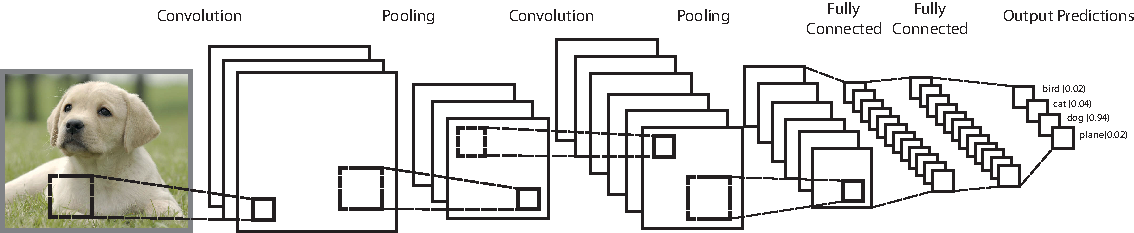
\includegraphics[width=1.1\linewidth]{figures/cnn.pdf}
\caption{Řetězec LeNet konvoluční neuronové sítě \cite{lenet}}
\label{fig:cnn}
\end{figure}
\section{Datasety chodců} 
V~průběhu let bylo shromážděno nespočet trénovacích sad pro chodce, které jsou veřejně dostupné na internetu. Všechny mají rozdílné charakteristiky, slabé a~silné stránky. 

Sada INRIA \cite{inria} patří mezi nejstarší sady. Ačkoliv obsahuje poměrně málo vzorků, přináší díky tomu vysokou kvalitu anotací chodců v~různých prostředích, což je většinou hlavní důvod, proč je tato sada vybrána pro trénování. Na rozdíl sady ETH \cite{eth} a~TUD-Brussels \cite{tudbrussels} patří mezi středně velké video sady. Další známou trénovací sadou je Daimler--Mono \cite{daimler}, kterou nelze použít pro všechny metodiky, poněvadž poskytuje vzorky v~odstínech šedi. Sady ETH, KITTI \cite{kitti} a~Daimler-Stereo \cite{daimlerstereo} poskytují stereofonní informace. Na obrázku \ref{fig:daimler_stereo} je ukázka tréninkové a~testovací sady Daimler-Stereo. 

\begin{figure}[H]
\centering
\includegraphics[width=16cm]{figures/daimler_stereo}
\caption{Ukázka trénovací a~testovací sady Daimler-Stereo \cite{daimlerstereo}}
\label{fig:daimler_stereo}
\end{figure}

V~dnešní době převládají Caltech-USA \cite{caltech} a~KITTI jako trénovací sady pro chodce. Obě poskytují poměrně velký počet vzorků. Caltech-USA vyniká počtem možných využití a~obsahuje více než 2300 jedinečných anotací chodců. KITTI zase předčí svou testovací sadou, která je více rozmanitější, ale na druhou stranu se tato sada nepoužívá tak často. V~roce 2014 vznikl projekt PETA (Pedestrian Attribute dataset)\cite{peta}. Tento projekt kombinuje mnoho trénovacích sad a~vytváří tak jednu velkou a~rozmanitou sadu, která usnadnuje učení robustních detektorů s~dobrým výkonem.

V~této práci používám převážně trénovací sadu CUHK01 \cite{cuhk}, sadu Das \cite{sudipdas} a~jako negativní sadu Daimler--Mono \cite{daimler}. Tato negativní sada se vyskytuje v~podobě fotografií zachycené kamerou při jezdě autem, bylo jí tedy nutné před použítím zpracovat. 


\section{Použité knihovny}
Na internetu je spousty dostupných či placených knihoven pro zpracování obrazu. Avšak nejznámější knihovnou pro zpracování obrazu je OpenCV. Dále jsem v práci použil knihovnu Dlib, která je taky dostupná na internetu a stále se vyvíjí. Obě tyto knihovny budou popsány v následující dvou kapitolách.
\subsection{Knihovna OpenCV}
OpenCV (\textit{Open Source Computer Vision Library}) je open-source knihovna, která slouží k~zpracování obrazu a~k~strojovému učení. Je psaná v~C/C++ jazyce s~podporou multijádrového zpracování.

Knihovna má více než 2500 optimalizovaných algoritmů, které zahrnují obsáhlé sady klasických a~moderních algoritmů pro zpracování obrazu a~strojové učení. Tyto algoritmy mohou být použity na detekci a~rozpoznávání tváří, identifikování objektů, vyhodnocování lidských akcí ve videosekvencích, sledování pohybů pomocí kamery, sledování pohybujících se objektů, extrahování 3D modelů z~objektů, vytváření 3D mračen bodů ze stereo kamer, spojování obrazu do jednoho s~vysokým rozlišením na dané scéně, hledání podobných obrazů z~obrazové databáze, odstranění červených očí z~obrazu způsobené bleskem, sledování pohybu očí, rozeznání scenérie a~vytvoření značek pro překrytí rozšířenou realitou a~další.

Knihovna má rozhraní pro jazyky C++, C, Python, Java a~MATLAB a~podporuje operační systémy Windows, Linux, Android, iOS a~MacOS. 
Pokud jsou dostupné MMX a~SSE instrukce tak knihovna je použije pro zvýšení jejího výkonu.

Podílí se na ní komunita lidí, kterou tvoří více než 47 tisíc uživatelů celého světa a~přesahuje více než 14 milionů stažení. 

%OpenCV leans mostly towards real-time vision applications and takes advantage of MMX and SSE instructions when available. A full-featured CUDA and OpenCL interfaces are being actively developed right now. There are over 500 algorithms and about 10 times as many functions that compose or support those algorithms. OpenCV is written natively in C++ and has a templated interface that works seamlessly with STL containers. 
%OpenCV (Open Source Computer Vision Library) is released under a BSD license and hence it’s free for both academic and commercial use. It has C++, C, Python and Java interfaces and supports Windows, Linux, Mac OS, iOS and Android. OpenCV was designed for computational efficiency and with a strong focus on real-time applications. Written in optimized C/C++, the library can take advantage of multi-core processing. Enabled with OpenCL, it can take advantage of the hardware acceleration of the underlying heterogeneous compute platform.

%Adopted all around the world, OpenCV has more than 47 thousand people of user community and estimated number of downloads exceeding 14 million. Usage ranges from interactive art, to mines inspection, stitching maps on the web or through advanced robotics.

Z~této knihovny byly použité následující nástroje:

\begin{itemize}
  \item{Mixtura Gausiánů,}
  \item{Konvexní obal,}
  \item{Histogram orientovaných gradientů,}
  \item{Support vector machines.}
\end{itemize}
\subsection{Knihovna Dlib}
Autorem této knihovny je Davis King. Jedná se o~moderní C++ knihovnu obsahující algoritmy pro strojové učení a~nástroje pro vytváření komplexních programů v~jazyce C++. Používá se jak v~industriálním tak v~akademické sféře v~široké škále oblastí. Jako jsou zejména vestavěná zařízení, robotika, mobilní telefony a~velkých, výkonných výpočetních prostředí. Jedná se o~sbírku nezávislých softwarových komponent z~nich každá je doprovázena důkladnou dokumentací a~mnoha příklady použítí.

Jádrem filozofie této knihovny je věnování snadnému používání a~přenositelnosti. Proto je kód navržen tak, aby nebylo po uživateli vyžadováno cokoli ručně konfigurovat nebo instalovat. K~dosažení tohoto cíle je veškerý kód specifický a~pro konkrétní platformu omezen a~obalen pomocí API rozhraní. Všechno ostatní je buď navrstveno na těchto obalech nebo napsané v~normě ISO standardu C++. 

Knihovna se stále rozrůstá hlavně díky dobrovolným přispěvovatelům a~konkrétně nyní obsahuje celou řadu užitečných nástrojů. Například softwarové komponenty pro práci se sítí, vlákna, grafické rozhraní, komplexní datové struktury, lineární algebra, statistické strojové učení, zpracování obrazu, data mining, XML a~parsování textu, numerická optimalizace, Bayeské sítě. V~uplynulých letech byla velká část vývoje zaměřena na širokou sadu nástrojů statického strojového učení, avšak knihovna zůstává univerzální.  

V~současné době je známo, že knihovna pracuje na systémech OS X, MS Windows, Linux, Solaris, BSD, HP-UX. Knihovna by měla také pracovat na libovolné platformě POSIX, ale není otestovaná na všech dostupných verzích. 
Z~této knihovny byl v~práci použit pouze FHOG detektor objektů.
%Knihovna Dlib je vyvíjena primárně Davidem Kingem, který je jejím autorem a její počátky tkví již v roce 2002. Tato knihovna je otevřená, multiplatformní a navržena designově na zakázku a komponenty jsou založeny na softwarovém inženýrství, jedná se o sbírku nezávislých softwarových komponent z nichž je každá doprovázena důkladnou dokumentaci a mnoha příklady použítí.


 
\section{Aplikace}
Aplikace je napsaná v nativní C++-14 ve vývojovém prostředí Visual Studio 2015. Jedná se o multiplatformní konzolovou aplikaci, která je primárně určena pro systémy ARM. 

Její obsluha je jednoduchá a funguje na bázi argumentů, které určují její chování. Nastavení parametrů se provádí přes externí soubor, což umožňuje jednodušší a pohodlnější manipulaci s aplikací. Disponuje širokým spektrem nástrojů od testování klasifikátorů, po jejich trénování až po samotnou detekci. Její nástroje jsou popsány v následujících podkapitolách.


 \begin{figure}[H]
\centering
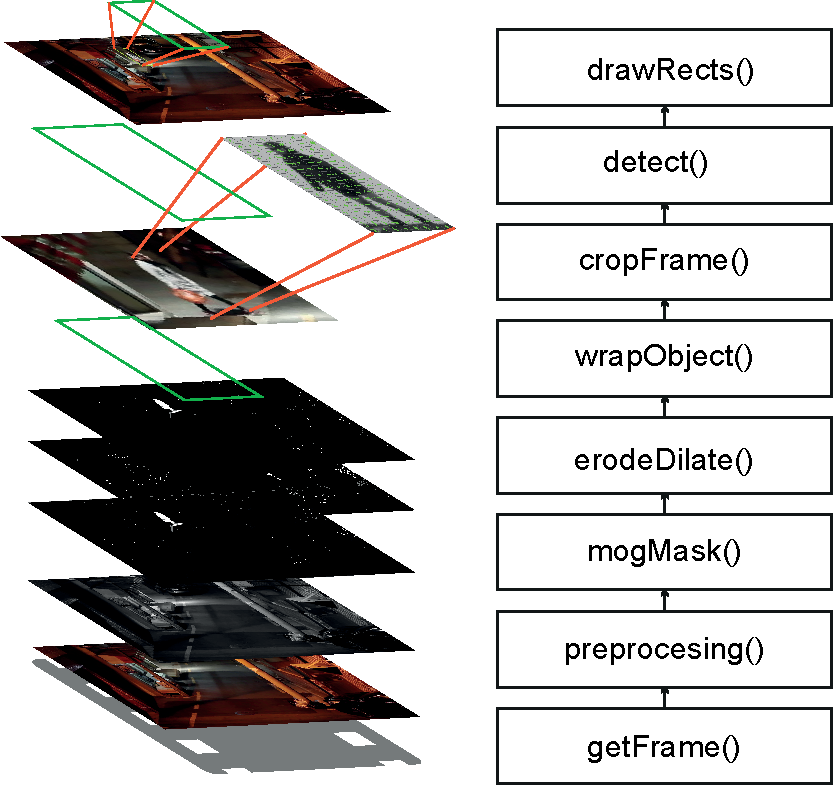
\includegraphics[width=14cm]{figures/alg_moghog}
\caption{Algoritmus aplikace při selekci kombinace MoG a HoG detekce}
\label{mog_algorithm}
\end{figure}

Obrázek \ref{mog_algorithm} ilustruje průběh algoritmu při volbě detekce pomocí HoGu a MoGu. Prvním krokem algoritmu je získání snímku z aktuální videosekvence nebo kamery, pokud obrázek je prázdný cyklus zde končí. Snímek se následně předzpracovává převodem do stupně šedi a aplikací rozostřovacího filtru. Tento obrázek je následně zpracováván metodikou substrakcí pozadí a na tento obraz se aplikuje eroze a dilatace, to proto, aby se v snímku vyfiltrovaly malé nevýznamné oblasti a následně spojily ty větší potencionální oblasti. Tyto oblasti se obalí kontury a převedou se na rámečky. Díky těmto rámcům se z obrazu vystřihnou a získáme výstřižky, na kterých v následujícím kroku probíhá samotná detekce. Detekční metoda vrátí rámce potencionálních oblastí chodců a vykreslí se do původního obrazu a proces se opakuje do té doby, pokud získaný obrázek z kamery není prázdný. Pokud obrázek po aplikování masky substrakce pozadí neobsahuje dostatečně velké oblasti k aplikaci rámců, program pokračuje načítáním dalšího rámce z kamery.  

\subsection{Testování klasifikátoru}
Testování klasifikátoru dle jejich parametrů vůči nějaké sadě negativních a pozitivních dat je nedílnou součástí vytvoření ideálního a úspěšného klasifikátoru.  Aplikace nabízí testování OpenCV a Dlib klasifikátoru. Diskriminační klasifikátor SVM z OpenCV lze testovat třemi způsoby. První a náhodný přístup je generování parametrů a různou iterací.

Další efektivnějším způsobem je testování pomocí diferenciální evoluce. Tento algoritmus vychází z genetického žíhání. Algoritmus nastaví určitý počet dimenzí pro testování parametrů SVM a následně probíhá ``žíhání'' parametrů takřka k jejich dokonalosti. Tento proces trvá 1000 cyklů.

Posledním druhem testování pro klasifikátor SVm z OpenCV je obdobné z Dlib knihovny, jedná se o vnořené cykly, kde se hrubou silou postupně testují parametry. 

Pro klasifikátor z Dlib knihovny je použita pouze metodika pro postupné testování parametrů hrubou silou v cyklech. Výhodou této metodiky je rozdělení trénovacích dat do 3 množin, kde dvě slouží na trénování a jedna pro testování a následně naopak. Toto testování trvá velice dlouho a výsledkem jsou přesnosti pro pozitivní a negativní množinu dat.


\subsection{Trénování klasifikátoru}
Program také umožňuje natrénování vlastního klasifikátoru. Parametry se vyberou z externího souboru s nastavením. V tomto souboru jsou také uloženy cesty k souborům se vzorky. 

Trénovací režim aplikace lze spustit přes argument '-t=train" a následně je uživateli nabídnut typ trénování. Program zvládne vytrénovat klasifikátor jak z knihovny OpenCV, tak i z knihovny Dlib. 

Trénování klasifikátorů z OpenCV probíhá naplněním vzorků do paměti včetně jejich kategorizace. Následně pro každý vzorek jsou vypočítané jeho vlastnosti a opět uložený do paměti programu. Posledním krokem před trénováním je jejich převod do jednořádkové matice a poté je spuštěno samotné trénování klasifikátorů. Tento krok trvá v závislosti na velikosti trénovací matice a zvolených parametrů. Uživatel může zvolit i dvojité trénování, za tímto stojí stejný postup, ale na konci trénování se spustí detekce pomocí posuvného okénka na negativních vzorcích a tyto vzorky budou rozšířeny o výstup z detektoru. Tento proces se nazývá Bootstraping. Výstupem trénování je soubor YAML, který je čitelný a slouží pro serializaci strukturovaných dat. Nalezneme zde parametry, použité pro trénování, vytrénované vzorky a vektor, který určuje rozdělující přímku.

Další možností je vytrénovaní klasifikátoru z knihovny Dlib. Trénování je obdobné jako u předchozí metody. Data jsou načtena jako mapy obrázků a tyto obrázky se parsují pomocí XML souboru. Trénování probíhá pouze z pozitivních vzorků a vychází z \cite{hog:dalal}. Výstupem je soubor s příponou dat.

Poslední možností trénování je kombinace výše zmíněných postupů. Vzorky se zpracují za pomocí OpenCV knihovny a vstupem do trénovací metody klasifikátoru z Dlibu je trénovací matice. Tu je nejprve nutné převést na formát této knihovny a poté je možné provést trénování.

Podstatný rozdíl mezi těmito binárními klasifikátory je v rozdílu jejich štítků. OpenCV klasifikátor můžeme definovat štítky libovolně, nejčastější však 1 pro pozitivní vzorky a 0 pro negativní. Zatím co Dlib klasifikátor přijímá pouze 1 pro pozitivní a zápornou 1 pro negativní vzorky.

Trénování klasifikátoru je velmi náročnou  operací na hardwarové prostředky. Ovšem závisí na trénovací sadě. Sada o počtu 200 tisíc vzorků zkonzumuje až 16 GB paměti.  Trénování kaskádového klasifikátoru je povoleno jen na  64-bitovém Windows, protože k trénování je využívána externí OpenCV aplikace. 

\subsection{Anotace chodců v obraze}
Aplikace také disponuje nástrojem pro anotaci chodců v obraze. Najednou umožňuje anotovat až 5 chodců a tyto anotace, i když to není až tak potřebné pro správnost anotace, jsou od sebe barevně odlišeny. Manipulace s tímto nástrojem je velmi snadná a jeho náhled je na obrázku \ref{tool_anotate}.

Klávesami `0' až `4' se přepíná mezi anotacemi, přičemž se tato selekce vypíše pro kontrolu do konzole. Klávesa `r' slouží pro vynulování vybrané anotace. Klávesou `n' přeskočíme aktuální snímek bez uložení anotovaných pozic. Klávesa `s' uloží aktuální anotované pozice do paměti a přepne se na další snímek, přičemž pozice první anotace zůstane nezměněná, to umožňuje jednodušší práci, pokud se v obraze nachází jen jeden chodec. Klávesy `i', `j', `k' a `l' umožňuje pohyb v obraze, pro přesnější umístění anotované části. Pokud tyto klávesy stiskneme společně s klávesou `shift', umožní nám to měnit velikost dané anotace. Klávesa `x' uloží aktuální pozice anotací v paměti do souboru. Tato funkcionalita umožňuje přerušovanou práci na anotacích videosekvence, ale vyžaduje manuální úpravu souboru uživatelem. Anotovaná část se může překrývat s jinou. Konkrétní anotace je zobrazena pro kontrolu samostatně zobrazena v dalším okně.

Všechny tyto oblasti zájmu a snímek s anotacemi jsou uloženy na disk v podobě obrázku pro pozdější kontrolu nebo oblasti zájmu mohou být použity pro trénování nebo cross validaci klasifikátoru. Výstup tohoto nástroje je plně kompatibilní s evaluační funkcí programu a jedná se tady o GroundTruth soubor všech anotací ve videosnímku.
 \begin{figure}[H]
\centering
\includegraphics[width=15cm]{figures/annotation_example}
\caption{Nástroj pro anotování oblastí chodců}
\label{tool_anotate}
\end{figure}

\subsection{Tvorba negativních vzorků z obrazu}
Tento nástroj umožňuje vytvořit negativní vzorky pro trénování procházením obrázku pomocí posuvného okénka. Velikost posuvného okénka je definována v externím souboru. Vstupem je textový soubor s cestami k obrázkům.

\section{ARM zařízení}
ARM systémy jsou kompletní počítače, vybudované na jedné desce s~procesorem, pamětí, vstupy, výstupy a~dalšími funkcemi. Jednodeskové počítače (\textit{SBC} - single-board computer) byly vyrobeny za účelem vývoje aplikací nebo jejich demonstraci, také slouží jako systémy pro vzdělávání nebo jsou použity jako vestavěné počítačové kontrolery. Typickým využitím těchto malých počítačů pro domácnost je její automatizace. 
Mezi známé a~výkonné můžeme zařadit následující vestavěné systémy.

\subsubsection*{Nvidia JETSON TK1}
Tento embedded systém disponuje nejen čtyřjádrovým procesorem Cortex-A15, ale i~grafickým čipem Nvidia Kepler s~192 Cuda jádry. Tato kombinace je jinak nazvaná jako Tegra K1 SoC (System on a~chip – integrovaný v~jediném obvodě). Tento procesor je údajně o~50\% výkonnější než Cortex-A9\footnote{https://developer.arm.com/products/processors/cortex-a/cortex-a15} a~podporuje instrukční sadu Armv7-A.

\subsubsection*{Asus Tinker Board}
Asus Tinker Board se řadí podle specifikace mezi ty výkonnější systémy. Na této desce se nachází čtyřjádrový procesor Cortex-A17 s~možností dynamického přetaktování (Turbo-Boost) až na 2,6 GHz. Tento počítač také podporuje instrukční sadu Armv7-A.  

\subsubsection*{Rock64}
Rock64 je produktem firmy Pine64 a~je osazen čtyřjádrovým procesorem Cortex-A53 a~až 4 GB operační paměti. Dále vyniká s~konektivitou USB 3.0 a~128 MB sériovou flash pamětí. Procesor podporuje instrukční sadu Armv8-A.

\subsubsection*{Odroid-XU4}
Tento počítač je vybaven osmijádrovým mobilním procesorem Samsung Exynos 5422. Tento procesor nabízí čtyřjádrový Cortex-A15 s~taktem 2,1 GHz a~další čtyřjádrový Cortex-A7 s~taktem 1,4 GHz. Což dělá tento počítač velmi výkonným na paralelní práci. Opět tento procesor podporuje instrukční sadu Armv7-A.

\subsubsection*{Intel Galileo}
Intel Galileo je prvním nízkoodběrovým produktem této firmy, disponuje jednojádrovým procesorem Intel Quark SoC X1000 s~taktem 400 MHz. První generace byla dostupná již v~roce 2013. Deska je navržena pro IoT (\textit{Internet of Things}) a~je zcela kompatibilní s~produkty, knihovny a~vývojovým prostředím elektrické platformy Arduino. 

\subsubsection*{Orange PI Plus 2E}
Orange PI je počítač velmi podobný Raspberry PI, ovšem svým výkonem je spíše obdobný počítači Banana PI. Orange PI Plus 2E je vybaven čtyřjádrovým procesorem Cortex-A7 s~podporou instrukční sady Armv7-A, 2 GB operační pamětí nebo například WiFi modulem s~anténou. Výhodou tohoto počítače je využití standardního DC konektoru k~napájení.

\subsubsection*{Cubieboard 5}
Tento počítač je osazen SoC čipem Allwinner H8. Jedná se o~symetrické osmijádro složené z~Cortex-A7 o~frekvenci 2,0 GHz. Dále na desce můžeme najít 2 GB operační paměti a~8 GB vestavěné úložiště. Tento embedded systém se od ostatních výše zmíněných liší tím, že na desce má osazený audio konektor S/PDIF a~DisplayPort, což umožnuje připojení až dvou monitorů a~také podporou RAID polí díky rozšiřující kartě. 

\subsection{Použitá zařízení}
K~otestování mého programu jsem využil počítače architektury ARM. Jedná se o~počítače SolidRun HummingBoard Pro, Raspberry PI 3 Model B a~Sinovoip Banana PI BPI-M1. Na těchto zařízeních bude otestován algoritmus a~všechny výsledky zapsány do tabulky v~následující kapitole.

\subsubsection*{HummingBoard Pro}
 Disponuje čtyřjádrovým procesorem i.MX6 Dual-core Lite na achitektuře Cortex A9 o~frekvenci 1 GHz, na desce má osazenou paměť typu DDR3 o~velikosti 2~GB a~nabízí grafický obvod Vivante GC880. Dále deska nabízí mSata konektor pro připojení SSD disku nebo například IR přijímač. Podporuje známé operační systémy Linux, například Android 4.4, Debian a~OpenSuse. Spotřeba zařízení je 2 W (0,41 A) v~klidovém stavu a~5 W (1 A) v~zátěži.

\subsubsection*{Raspberry PI 3}
Jedná se o~třetí generaci velmi úspěšné řady Raspberry PI. Model je osazen výkonným 64 bitovým čtyřjádrovým procesorem Cortex-A53 o~frekvenci 1,2 Ghz, grafickým čipem Broadcom VideoCore IV o~frekvenci 400 MHz, operační paměť typu SDRAM o~velikosti 1GB, která je sdílená s~grafickým čipem. Od svých předchůdců se líší integrovaným Wifi čipem podporující protokoly 802.11 b/g/n a~Bluetooth 4.1 LE. Díky architektuře ARMv8 má šiřší podporu Linuxů, včetně mobilního systému Android a~Windows 10 IoT. Jeho výkon bez zátěže je 1,5 W (300 mA) a~při zátěži se zapojenými periferiemi maximálně 6,7 W (1,34 A).

\subsubsection*{Banana PI}
Tento počítač je osazen dvoujádrovým procesorem AllWinner A20 s~frekvencí 1,2 GHz. Jedná se o~low-end verzi procesoru AllWinner A31. Dále na desce najdeme grafický čip Mali-400 MP2 a~operační paměť 1 GB. Jedná se o~první klon RPI a~jeho deska je osazena navíc například sata konektorem, mikro-USB OTG nebo mikrofonem. Tento mikropočítač díky GLAN můžeme použít jako vzdálené NAS úložiště (\textit{Network Attached Storage}), databázi, mail server nebo například web server. Jeho spotřeba v~nečinném stavu je 1,75 W (350 mA), maximálně 5.5 W (1,1 A).

\subsection{Srovnání použitých zařízení}
Jedná se o~poměrně výkonné počítače vzhledem ke své velikosti. V~následující tabulce se nachází srovnání některých parametrů těchto počítačů.
\begin{table}[H]
\centering
\caption{Srovnání testovaných zařízení}
\begin{tabular} { |c|c|c|c| }
\hline
{}                  & {HummingBoard Pro}    & {Raspberry PI 3}      & {Banana PI}          \\ \hline
Procesor            & NXP i.MX6 ARM         & ARM                   & A20 ARM              \\ \hline
Počet jader         & 4                     & 4                     & 2                    \\ \hline
Kmitočet            & 1 GHz                 & 1,2 GHz               & 1,2 GHz              \\ \hline
Druh architektury   & Cortex A9             & Cortex A53            & Cortex A7            \\ \hline
Grafický čip        & Vivante GC880         & BroadCom VideoCore IV & Mali-400 MP2         \\ \hline
Kapacita paměti RAM & 1 GB                  & 1 GB                  & 1 GB                 \\ \hline
Druh paměti         & DDR3                  & LPDDR2                & DDR3                 \\ \hline
Ethernet            & 10/100/1000           & 10/100                & 10/100/1000          \\ \hline
Počet USB portů     & 2                     & 4                     & 2                    \\ \hline
Úložný prostor      & MicroSD               & MicroSDHC             & SD/MMC               \\ \hline
Rok vydání          & 2014                  & 2016                  & 2014                 \\ \hline
\end{tabular}
\label{srovnaniPC}
\end{table}

\section{Experimenty}

Experimenty této práce probíhaly především na počítačích uvedených v~předchozí kapitole. Nejprve je však vhodné zmínit konfiguraci daných počítačů:
\begin{itemize}
\item\textbf{HummingBoard Pro} - na tomto počítači je nainstalován Linux Debian 8.1 s~označením ``jessie'' s~grafickým rozhraním MATE 8.
\item\textbf{Banana PI} - na tomto počítači je nainstalován Linux Debian 8.1 s~označením ``jessie'' s~grafickým rozhraním Xfce 4.10. 
\item\textbf{Raspberry PI} - na tomto počítači je nainstalován Linux Raspbian. 
\end{itemize}
Dále pro srovnání výkonu těchto počítačů byl program otestován i~na desktopovém počítači, na kterém byl zároveň vyvíjen a~odladěn. Jeho parametry jsou následující: 
\begin{itemize}
\item\textit{Intel Core i7--6700k}, operační paměť  \textit{32 GB} a~operační systém  \textit{Windows 10 Pro}.
\end{itemize}
První sada experimentů byla detekce pomocí histogramů orientovaných gradintů a~jeho vylepšení pomocí algoritmu pro substrakci pozadí při detekci ze statických kamer.

\subsection{Nalezení optimálního klasifikátoru}

Nalezení optimálního a~spolehlivého klasifikátoru je klíčovou částí celého procesu, zároveň se jedná i~o~velmi komplikovaný a~zdlouhavý úkol. Je důležité zvolit ideální tréninkovou sadu vzorků a~k~vzhledem zvoleného typu SVM a~jejího jádra. Otestoval jsem varianty $C$, $\nu$, $\varepsilon$--SVR klasifikátorové typy s~lineárním a~Gaussovým jádrem, přičemž jsem zjistil, že nejlepší sestava pro detekování chodců je kombinace typu $\varepsilon$--SVR s~lineárním jádrem, protože pozitivní detekce byla poměrně větší než negativní. Při zvolení správného jádra a~typu klasifikátoru je dalším krokem vybrat, jak už bylo zmíněno, tréninkovou sadu. Vyzkoušel jsem nejrůznější tréninkové sady dostupné na internetu a~jejich kombinace.

Nejlepších výsledků jsem dosáhl s~pozitivní trénovací sadou Dase \cite{sudipdas}, CUHK01 campus \cite{cuhk} a~jako negativní sadu jsem použil Daimler--Mono\cite{daimler}, kterou jsem nastříhal na vzorky. Tyto sady jsou přiloženy v~příloze této práce. Následujícím krokem je zvolení správných parametrů trénování klasifikátoru. 

Trénování klasifikátoru je velmi citlivé na tyto parametry, při změně některého z~nich jen o~tisícinu, můžeme získat úplně jiný výsledek. Trénování probíhalo dvakrát za sebou. Při druhém trénování se klasifikátor učil ze svých špatných detekcí, čemuž se říká ``Bootstrapping''. To znamená, že detekce se spustila na negativních vzorcích s~tímto klasifikátorem a~pokud detektor vrátil nějaký výsledek, byl zpět uložen do negativní sady a~znovu natrénován, tento postup je ilustrován ve zdrojovém kódu \ref{src:double_train}.
\newpage

\begin{lstlisting}[label=src:double_train, language=cpp, caption=Bootstrapping]
		cv::Size posSize = posSamplesLst[0].size();
		cv::HOGDescriptor myHog;
		myHog.winSize = posSize;
		std::vector < cv::Rect > locations;
		std::vector < float > hogDetector;
		
		getSvmDetector(svm, hogDetector);
		myHog.setSVMDetector(hogDetector);

		std::vector < cv::Rect > detections;

		for (size_t i~= 0; i~< negSamplesLst.size(); i++)	{
			myHog.detectMultiScale(negSamplesLst[i], detections);
			for (size_t j = 0; j < detections.size(); j++)	{
				cv::Mat detection = negSamplesLst[i](detections[j]).clone();
				resize(detection, detection, posSize);
				negSamplesLst.push_back(detection);
			}
		}
		labels.clear();
		labels.assign(posSamplesLst.size(), +1);
		labels.insert(labels.end(), negSamplesLst.size(), 0);

		gradientLst.clear();
		extractFeatures(posSamplesLst, gradientLst);
		extractFeatures(negSamplesLst, gradientLst);

		convertSamples2Mat(gradientLst, trainMat);
		trainSvm(trainMat, labels);
\end{lstlisting}

Natrénoval jsem klasifikátory s~různými parametry a~otestoval je na testovacích vzorcích. Tyto vzorky byly vyextrahované obrázky chodců a~"ne-chodců" z~testovacích videí pomocí jejich anotací a~přiloženého nástroje pro tvorbu vzorků a~také z~projektu PETA, konkrétně se jednalo o~sady: \textit{3DPeS, CAVIAR4REID, CBLC, SARC3D a~VIPeR}\cite{peta}. Tento krok je v~podstatě první filtrací klasifikátorů. Vybíráme takový klasifikátor, aby jeho detekce byla co nejvíc přesná a~detekoval, co nejméně špatných oblasti. Vytrénoval jsem 15 klasifikátorů s~různými parametry trénování. Tyto klasifikátory jsem nadále filtroval pomocí ROC křivky a~vizuálně vybral ten nejlepší z~obrázku \ref{fig:rocCurve1}.  Nastavení trénovacích parametrů jsou uvedeny v~tabulce \ref{classTab1}.  

\begin{figure}[H]
\centering
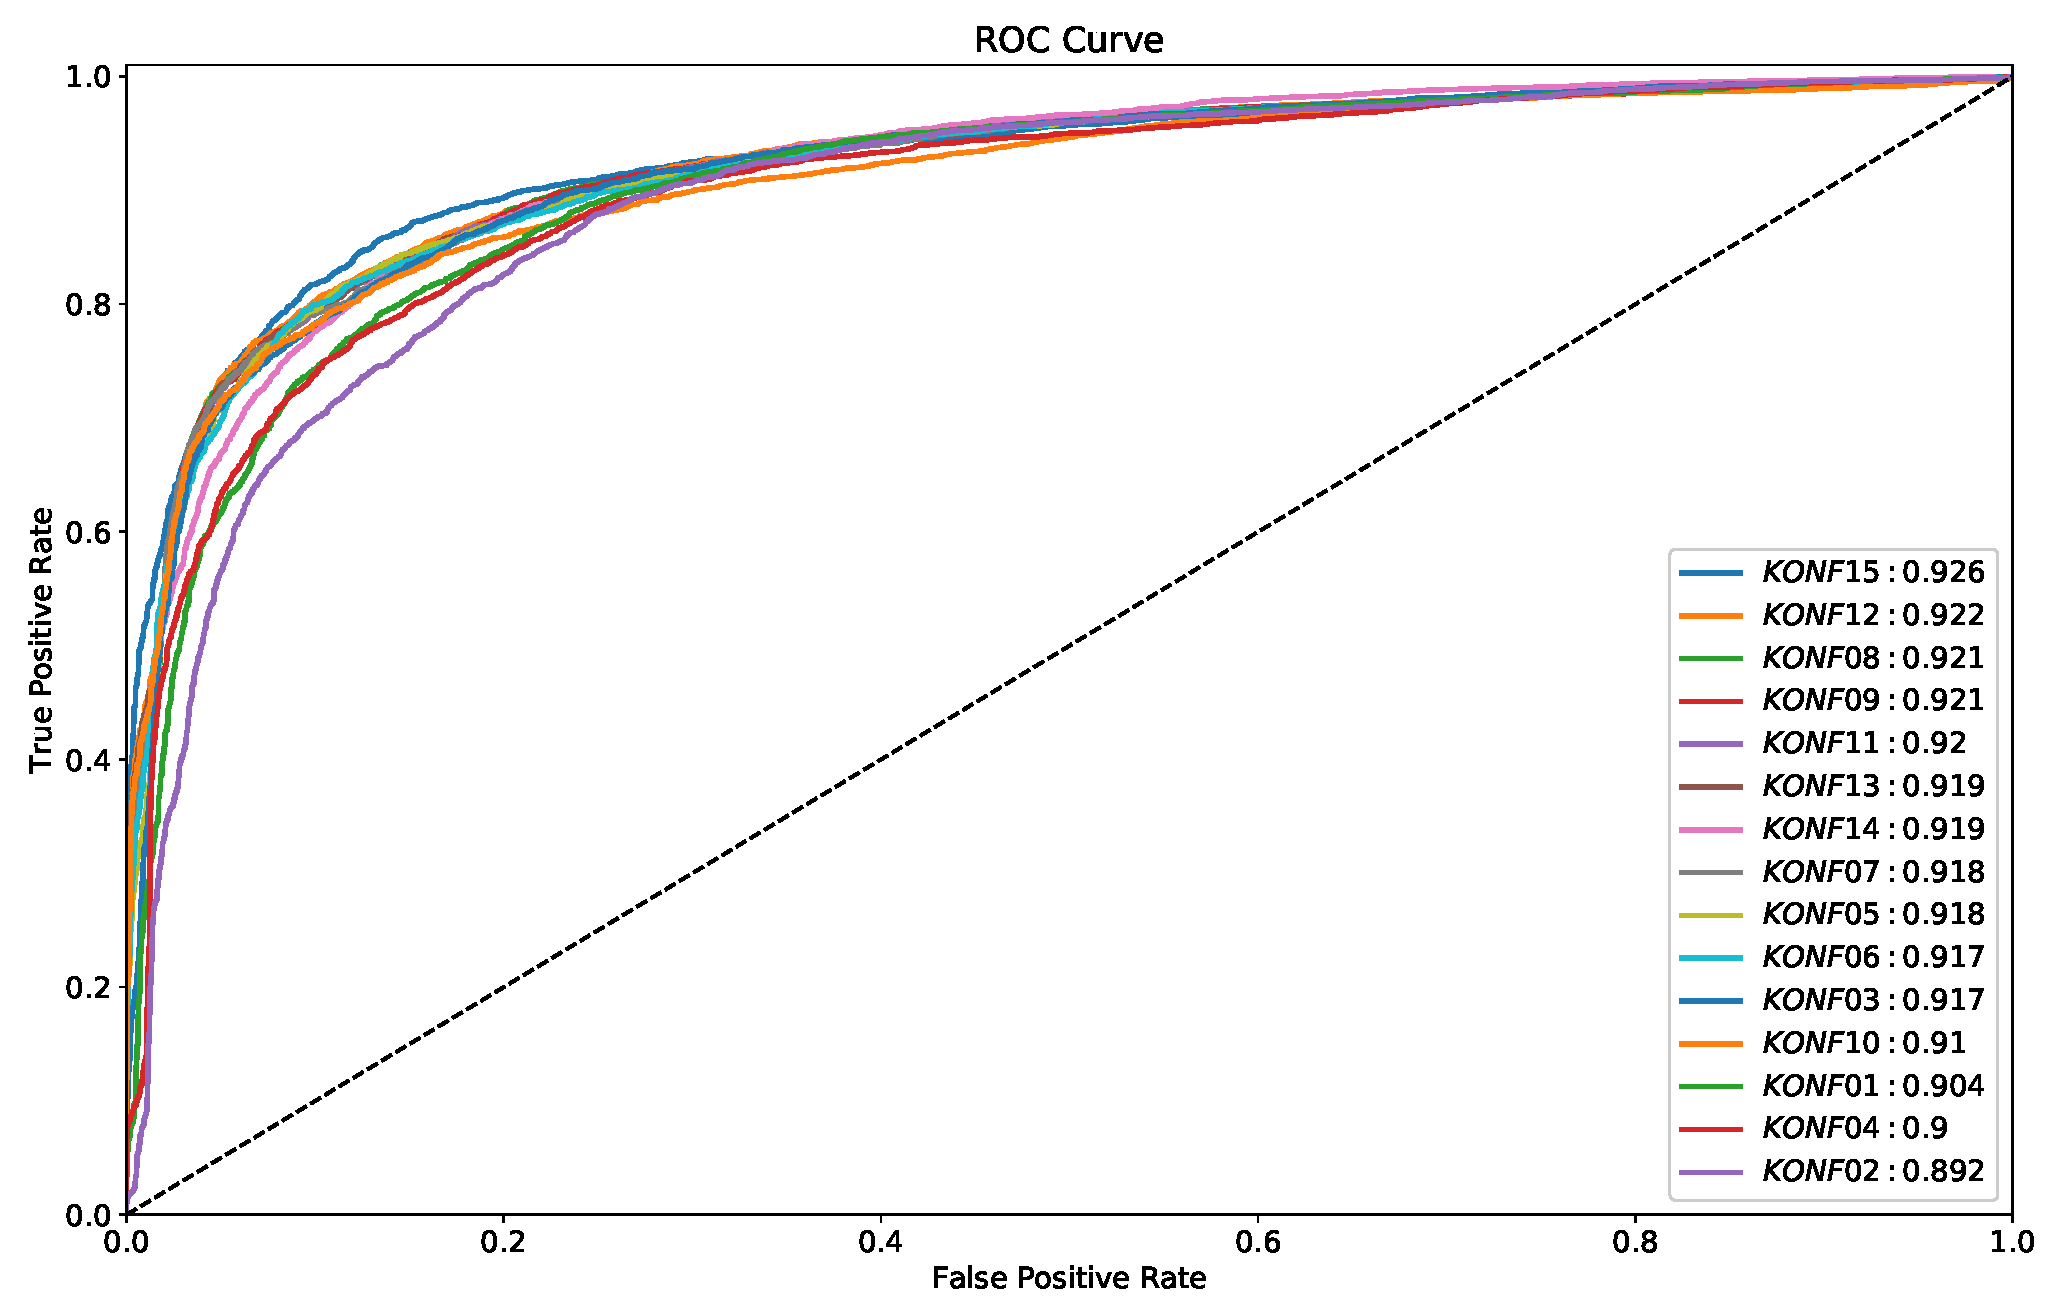
\includegraphics[width=16cm]{figures/roc1}
\caption{ROC křivka natrénovaných klasifikátorů}
\label{fig:rocCurve1}
\end{figure}

\begin{table}[H]
\centering
\caption{Přehled vytrénovaných klasifikátorů a~jejich trénovacích parametrů. Parametry $\varepsilon$, kritéria ukončení a~počet pozitivních vzorků (5649) byly stejné.}
\begin{tabular} { |c|c|c|c|c|c| }
\hline
{}             & {par. C}     & {par. P}      & {max iterací} & {počet neg. vzorků} & {Přesnost \%}  \\ \hline
KONF 01		& 	0.005	& 	  0.02	 &   2000   	  &		  3000   	    &        83	 \\ \hline
KONF 02		& 	0.005	& 	  0.01	 &   3500   	  &		  3000   	    &        81	 \\ \hline
KONF 03		& 	0.001	& 	  0.02	 &   2000   	  &		  6000   	    &        83	 \\ \hline
KONF 04		& 	0.001	& 	  0.02	 &   4500   	  &		  6000   	    &        81	 \\ \hline
KONF 05		& 	0.005	& 	  0.4 	 &   3500   	  &		  6000   	    &        84	 \\ \hline
KONF 06		& 	0.01 	& 	  0.4 	 &   3000   	  &		  6000   	    &        84	 \\ \hline
KONF 07		& 	0.005	& 	  0.01	 &   2500   	  &		  9000   	    &        82	 \\ \hline
KONF 08		& 	0.005	& 	  0.25	 &   2000   	  &		  9000   	    &        82	 \\ \hline
KONF 09		& 	0.005	& 	  0.25	 &   3000   	  &		  9000   	    &        82	 \\ \hline
KONF 10 	     & 	0.01 	& 	  0.02	 &   3000   	  &		  9000   	    &        80	 \\ \hline
KONF 11 	     & 	0.01 	& 	  0.25	 &   2000   	  &		  9000   	    &        82	 \\ \hline
KONF 12 	     & 	0.01 	& 	  0.25	 &   2500   	  &		  9000   	    &        82	 \\ \hline
KONF 13 	     & 	0.01 	& 	  0.25	 &   4500   	  &		  9000   	    &        82	 \\ \hline
KONF 14 	     & 	0.5	 	& 	  0.1	 &   1200   	  &		  9000   	    &        81	 \\ \hline
KONF 15 	     & 	0.5		& 	  0.1	 &   2000   	  &		  9000   	    &        83	 \\ \hline
\end{tabular}
\label{classTab1}
\end{table}

Vybral jsem konfiguraci 15, protože oblast pod křivkou byla největší ze všech natrénovaných, přesnost tohoto klasifikátoru je v~tabulce \ref{classTab2}. Výsledky testování ostatních klasifikátorů jsou v~příloze této práce. Detekce může nabývat maximálně 4 stavů:
\begin{itemize}
	\item{True Positive (\textbf{TP}) - detektor správně rozpoznal chodce.}
	\item{True Negative (\textbf{TN}) - detektor tuto oblast ignoroval.}
	\item{False Positive (\textbf{FP}) - detektor označil tuto oblast za chodce, ovšem se zde nenachází.}
	\item{False Negative (\textbf{FN}) - v~oblasti se vyskytuje chodec avšak byl ignorován.}
\end{itemize}

Díky těmto stavům můžeme vypočítat přesnost detekce:
\begin{equation*}
\centering
 \label{eq:accuracy}
 \begin{aligned}
Accuracy = \frac{TP + TN}{TP + TN + FP + FN}
 \end{aligned}
\end{equation*}

\begin{table}[H]
\centering
\caption{Přesnost konfigurace klasifikátoru číslo 15}
\begin{tabular} { |c|c|c|c|c| }
\hline
{}          & {TP/FN} 	 & {TN/FP} 	& {Přesnost \%} & {AUC}  \\ \hline
KONF 15 	&  3479/1572 & 4912/192 &     83 		& 0.926  \\ \hline
\end{tabular}
\label{classTab2}
\end{table}
Na tento klasifikátor jsem se rozhodl aplikovat algoritmus substrakce pozadí, a~tak zefektivnit jeho rychlost a~správnost detekce na videosekvenci ze statické kamery.

\subsection{Aplikace algoritmu Mixtura Gaussiánů}
V~předchozí kapitole jsem popsal, jak probíhalo zvolení optimálního klasifikátoru a~nyní jej použijeme na reálná data. Chodci jsou v~použitých videosekvencích a~obrázcích anotováni v~textových souborech každý zvlášť. První řádek tohoto textového souboru odpovídá počtu snímku videa a~další řádky jsou věnovány samotným anotacím, kde první číslo vyjadřuje číslo snímku a~následující 4 čísla jsou body dané anotace.

Testovací video je ve 3 druzích rozlišení, základní informace o~videosekvencích je uvedena v~tabulce \ref{videosTab}, rozdíl mezi výskytem osob a~snímků za sekundu je způsobené převodem videa.

\begin{table}[H]
\centering
\caption{Přehled testovaných videozáznamů}
\begin{tabular} { |c|c|c|c|c| }
\hline
{Název videa}   & {Rozlišení} 	&   {Počet snímků}  & {FPS} & {Výskyt osob na snímcích} \\ \hline
cctv4.mp4 	 &  640 x  360	     &      781		& 29,97 & 	      754			 \\ \hline
cctv4.avi		 & 1280 x  720	     &      626		& 24,00 & 	      597			 \\ \hline
cctv4.mov 	 & 1920 x 1080	     &      781		& 29,97 & 	      749			 \\ \hline
\end{tabular}
\label{videosTab}
\end{table}

Chodci se ve videosekvenci mohli vyskytovat kdekoliv, proto se při takové detekci používá výpočet F1--skóre namísto přesnosti. Ke svému výpočtu totiž nepotřebuje true negative, které by bylo snad nemožné získat z~každého snímku. Výpočet F1--skóre je následující
\begin{equation*}
\centering
 \label{eq:f1score}
 \begin{aligned}
F1-score = \frac{ 2TP}{2TP + FP + FN}
 \end{aligned}
\end{equation*}

Také jsem stanovil pravidlo pro pozitivní detekci a~to takové, že výstup z~detektoru je považován za pozitivní právě tehdy, když jeho plocha je větší než polovina anotované plochy. 

Navzdory tomu, že tyto počítače podporují rozšíření NEON a~obě knihovny byly kompilovány s~tímto rozšířením, výsledky nebyly až tak časově uspokojivé, jak jsem očekával. V~následujících tabulkách jsou uvedeny výsledky detekce mého vytrénovaného detektoru. Také jsou zde uvedeny výsledky detektoru z~knihovny Dlib včetně původního detektoru lidí, který je obsažen v~OpenCV (v~tabulkách je zaznamenán jako ``default'') a~slouží k~porovnání k~detektoru s~vytrénovaným SVM klasifikátorem. 

V~tabulkách \ref{resultTabIMX}, \ref{resultTabRPI3} a~\ref{resultTabBPI} jsou uvedeny výsledky detekce z~každého videa na jednotlivém zařízení. Tabulka \ref{resultTabDesktop} jsou výsledky z~desktopového počítače, které slouží jako referenční model k~výsledkům z~výše zmíněných tabulkách.  
\begin{table}[H]
\catcode`\-=12
\centering
\caption{Výsledky detekce počítače HummingBoard Pro i.MX6 }
\label{resultTabIMX}
\begin{tabular}{|c|c|c|c|c|c|c|c|}
\hline
                         & Typ algoritmu   	& ALG FPS & Délka detekce [s] & TP  & FN  & FP  & F1--skóre [\%] \\ \hline
\multirow{6}{*}{cctv4.mp4} & HOG        	&   0,9   &      832,2        & 447 & 307 & 164 &    65          \\ \cline{2-8} 
                         & HOG + MOG  		&   4,5   &      172,5        & 550 & 204 & 17  &    83          \\ \cline{2-8}  
                         & FHOG       		&         &                   &     &     &     &                \\ \cline{2-8}  
                         & FHOG + MOG 		&         &                   &     &     &     &                \\ \cline{2-8}  
                         & default	 		&   0,7   &      856,9        & 297 & 457 & 27  &    55          \\ \cline{2-8}  
                         & default + MOG	&   2,1   &      303,1        & 558 & 39  & 73  &    91          \\ \hline\hline 
\multirow{6}{*}{cctv4.avi} & HOG        	&   0,6   &     1010,9        & 416 & 181 &  15 &    81          \\ \cline{2-8} 
                         & HOG + MOG  		&   1,1   &      527,3        & 477 & 120 & 15  &    87          \\ \cline{2-8}  
                         & FHOG       		&      &              &  &  &   &          \\ \cline{2-8} 
                         & FHOG + MOG 		&         &                   &     &     &     &          \\ \cline{2-8} 
                         &  default 		&         &                   &     &     &     &          \\ \cline{2-8}  
                         & default + MOG	&         &                   &     &     &     &          \\ \hline \hline
\multirow{6}{*}{cctv4.mov} & HOG        	&         &                   &     &     &     &          \\ \cline{2-8} 
                         & HOG + MOG  		&         &                   &     &     &     &          \\ \cline{2-8} 
                         & FHOG       		&         &                   &     &     &     &          \\ \cline{2-8}  
                         & FHOG + MOG 		&         &                   &     &     &     &          \\ \cline{2-8} 
                         & default 		&         &                   &     &     &     &          \\ \cline{2-8} 
                         & default + MOG 	&         &                   &     &     &     &          \\ \hline
\end{tabular}
\end{table}


\begin{table}[H]
\catcode`\-=12
\centering
\caption{Výsledky detekce počítače Raspberry PI3}
\label{resultTabRPI3}
\begin{tabular}{|c|c|c|c|c|c|c|c|}
\hline
                         & Typ algoritmu 	& ALG FPS & Délka detekce [s] & TP 		& FN 	& FP 	& F1--skóre [\%]  \\ \hline
\multirow{6}{*}{cctv4.mp4} & HOG         	&   1,2   &   661,6       	  & 441   	& 313     & 158     &    65           \\ \cline{2-8} 
                         & HOG + MOG  		&   4,8   &   164,7       	  & 579		& 175  	& 18   	& 	86	        \\ \cline{2-8} 
                         & FHOG       		&         &   			  &    		&    	&    	& 		        \\ \cline{2-8} 
                         & FHOG + MOG 		&         &               	  &    		&    	&    	& 		        \\ \cline{2-8} 
                         & default	 		&   1,1   &   722,2             & 297   	& 457   	& 26    	&    55 		   \\ \cline{2-8} 
                         & default + MOG 	&   2,9   &   273,9 		  & 365   	& 389    	&  1		&    65           \\ \hline\hline 
\multirow{6}{*}{cctv4.avi} & HOG      		&   0,8   &   799,7        	  & 417   	& 183 	& 15      & 	81	        \\ \cline{2-8} 
                         & HOG + MOG  		&   1,2   &   508,4       	  & 475		& 122 	& 15   	& 	87	        \\ \cline{2-8} 
                         & FHOG       		&         &               	  &    		&    	&    	& 		        \\ \cline{2-8} 
                         & FHOG + MOG 		&         &               	  &    		&    	&    	& 		        \\ \cline{2-8} 
                         & default	 		&         &               	  &    		&    	&    	& 		        \\ \cline{2-8} 
                         & default + MOG 	&         &               	  &    		&    	&    	& 		        \\ \hline \hline
\multirow{6}{*}{cctv4.mov} & HOG      		&   0,4   &   2 091,1      	  & 556 	     & 193 	& 156  	& 	76	        \\ \cline{2-8} 
                         & HOG + MOG  		&   0,4   &   1 944,8      	  & 547		& 202  	& 56	     & 	81	        \\ \cline{2-8} 
                         & FHOG       		&         &               	  &    		&    	&    	& 		        \\ \cline{2-8} 
                         & FHOG + MOG 		&         &               	  &    		&    	&    	& 		        \\ \cline{2-8} 
                         & default	 		&         &               	  &    		&    	&    	& 		        \\ \cline{2-8} 
                         & default + MOG 	&         &               	  &    		&    	&    	& 		        \\ \hline
\end{tabular}
\end{table}


\begin{table}[H]
\catcode`\-=12
\centering
\caption{Výsledky detekce počítače Banana PI BPI-M1}
\label{resultTabBPI}
\begin{tabular}{|c|c|c|c|c|c|c|c|}
\hline
                         & Typ algoritmu	& ALG FPS & Délka detekce [s] & TP 	  & FN 	& FP 	& F1--skóre [\%] \\ \hline
\multirow{6}{*}{cctv4.mp4} & HOG      		&  0,4    &   1 795,5    	  & 437   & 317 & 157  	&   65     	 	  \\ \cline{2-8} 
                         & HOG + MOG  		&  2,9    &     267,5     	  & 577   & 177 & 15  	&   86     		  \\ \cline{2-8} 
                         & FHOG       		&         &               	  &    &    &    &          \\ \cline{2-8} 
                         & FHOG + MOG 		&         &               	  &    &    &    &          \\ \cline{2-8}  
                         & default	 		&  0,4    &    1760,3           & 299   & 455 & 24     &   55                \\ \cline{2-8}  
                         & default + MOG 	&  1,4    &     548,5           & 364   & 390 & 3      &   65                \\ \hline\hline 
\multirow{6}{*}{cctv4.avi} & HOG        	&  0,3    &   1 909,3     	  & 416	& 181 & 13   &   81     		       \\ \cline{2-8} 
                         & HOG + MOG  		&  0,8    &     739,4      	  & 470   & 127 & 20   &   86                  \\ \cline{2-8} 
                         & FHOG       		&         &               	  &    &    &    &          \\ \cline{2-8} 
                         & FHOG + MOG 		&         &               	  &    &    &    &          \\ \cline{2-8} 
                         & default	 		&         &               	  &    &    &    &          \\ \cline{2-8} 
                         & default + MOG 	&         &               	  &    &    &    &          \\ \hline \hline
\multirow{6}{*}{cctv4.mov} & HOG        	&  0,14   &   5 718,8     	  & 572	  & 177  & 114  &   80		    \\ \cline{2-8} 
                         & HOG + MOG  		&  0,21   &   3 709,5      	  & 544   & 205  & 66   &   80          \\ \cline{2-8} 
                         & FHOG       		&         &               	  &    &    &    &          \\ \cline{2-8} 
                         & FHOG + MOG 		&         &               	  &    &    &    &          \\ \cline{2-8} 
                         & default	 		&         &               	  &    &    &    &          \\ \cline{2-8} 
                         & default + MOG 	&         &               	  &    &    &    &          \\ \hline
\end{tabular}
\end{table}

\begin{table}[H]
\catcode`\-=12
\centering
\caption{Výsledky detekce desktopového počítače}
\label{resultTabDesktop}
\begin{tabular}{|c|c|c|c|c|c|c|c|}
\hline
                         & Typ algoritmu   	& ALG FPS & Délka detekce [s] & TP 	& FN & FP & F1--skóre [\%]\\ \hline
\multirow{6}{*}{cctv4.mp4} & HOG        	&  20,8   & 37,5       		  & 463 & 291   & 135   &  68        \\ \cline{2-8} 
                         & HOG + MOG  		& 128,03  &  6,1       		  & 584 & 170    & 12    & 87          \\ \cline{2-8} 
                         & FHOG       		&         &            		  &     &    &    &          \\ \cline{2-8} 
                         & FHOG + MOG 		&         &            		  &     &    &    &          \\ \cline{2-8}  
                         & default	 		&  21,1   & 37,07               & 304 & 450    & 27    & 56          \\ \cline{2-8} 
                         & default + MOG 	&  48,9   & 12,8                & 374 & 380    & 4    & 66          \\ \hline\hline 
\multirow{6}{*}{cctv4.avi} & HOG        	& 13,1    & 47,6           	  &  410& 187   & 18    & 80          \\ \cline{2-8} 
                         & HOG + MOG  		&   34,4  & 18,2          	  & 484 & 113    & 14    & 88          \\ \cline{2-8} 
                         & FHOG       		&         &               	  &    	&    &    &          \\ \cline{2-8} 
                         & FHOG + MOG 		&         &               	  &    	&    &    &          \\ \cline{2-8} 
                         & default  		& 4,3     & 144,8               & 554 & 43     & 60    & 91          \\ \cline{2-8} 
                         & default + MOG 	& 30,8    & 20,3                & 344 & 253    & 14    & 72          \\ \hline \hline
\multirow{6}{*}{cctv4.mov} & HOG        	& 5,6     & 138,7               &  560& 189    & 133    & 78          \\ \cline{2-8} 
                         & HOG + MOG  		& 8,4     & 92,6                & 568& 181    & 47    & 83          \\ \cline{2-8} 
                         & FHOG       		&         &               	  &    	&    &    &          \\ \cline{2-8} 
                         & FHOG + MOG 		&         &                     &    	&    &    &          \\ \cline{2-8} 
                         & default  		& 1,7     & 451,6               & 706   & 43    & 507    & 72          \\ \cline{2-8} 
                         & default + MOG 	& 13,7    &  56,9               & 386   & 363    & 86    & 63          \\ \hline
\end{tabular}
\end{table}

V~obrázku \ref{fig:rocCurve2} jsou vykresleny ROC křivky všech tří videí za použití kombinace metod MOG a~HOG. Tyto křivky byly vygenerovány obdobně jako při testování klasifikátoru. SVM klasifikátor na každé detekci provedl pravděpodobnostní zařazení do konkrétní třídy, jinými slovy, jestli se na obrázku nachází chodec nebo nikoliv. V~posledním kroku se vygeneroval Ground truth soubor k~tomuto pravděpodobnostnímu ohodnocení za pomocí anotačního souboru. Jak může být zřejmé, klasifikátor není až tak spolehlivý na obsah s~vysokým rozlišením, na druhou stranu detekci na průměrném rozlišení (720p) je spolehlivější. Natrénoval jsem klasifikátor na vzorcích o~velikosti $48x96$ pixelů proto, aby bylo možné detektor použít i~na menších obrázcích bez nutnosti zvětšování obsahu.   

\begin{figure}[H]
\centering
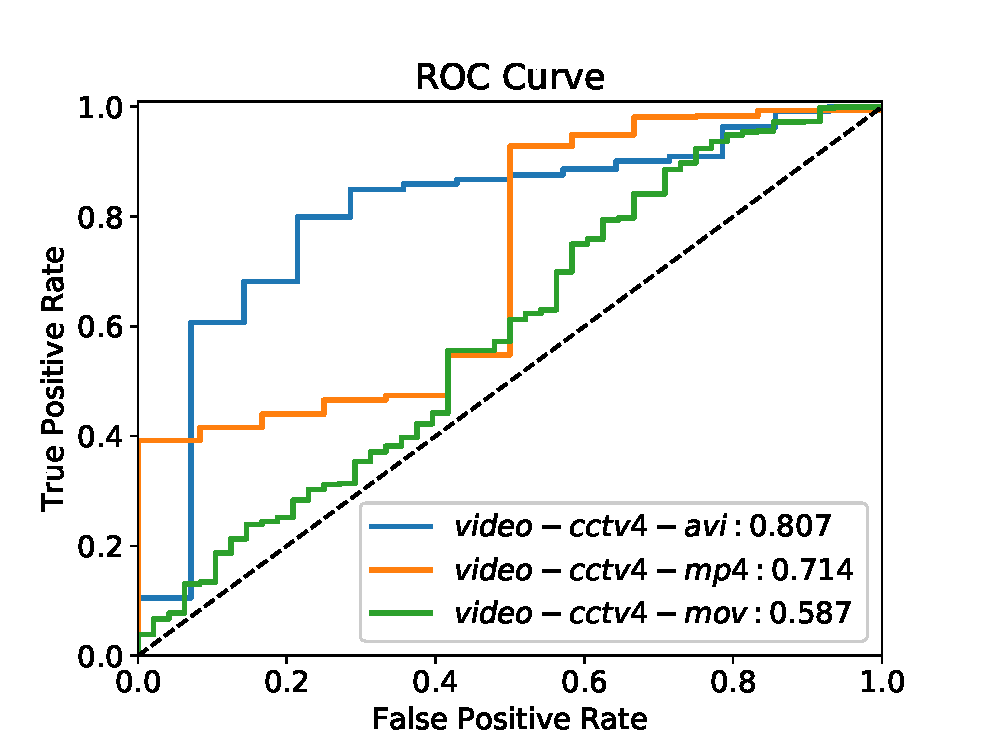
\includegraphics[width=16cm]{figures/roc2}
\caption{ROC křivky klasifikátoru na videosekvencích z~tabulky \ref{videosTab}}
\label{fig:rocCurve2}
\end{figure}

Předfiltrování obrazu pomocí subtrakce pozadí se projevilo jako užitečná metodika pro detekci chodců. Nejen, že se zefektivnila detekce odfiltrováním většiny false positive, ale také rychlost samotného algoritmu, například na dvoujádrovém počítači Banana Pi je rychlost skoro až $7x$ rychlejší než bez substrakce pozadí při nízkém rozlišení videa.  

\section{Závěr}
Dle zadání práce byly otestované vybrané metodiky z knihoven OpenCV a Dlib pro rozpoznávání chodců. Z těchto metodik byly vybrány algoritmy z OpenCV - Histogram orientovaných gradientů, kaskádové klasifikátory a z Dlib knihovny byl vybrán Histogram orientovaných gradientů a tyto algoritmy byly implementovány v aplikaci. Obě tyto knihovny disponují nástroji pro natrénování klasifikátoru, které se dají poté použít na samotnou detekci.

Trénování klasifikátoru hraje důležitou roli pro samotnou detekci, protože zvyšuje přesnost detekce a účinnost klasifikátoru.  Další významnou roli na samotnou úspěšnost klasifikátoru je množina trénovacích dat a nastavení trénování klasifikátoru. Tato data by měla být co nejpřesnější a obsahovat minimum stínu a minimum artefaktů. Jak bylo již v tomto dokumentu zmíněno, aplikace obsahuje i nástroje pro otestování klasifikátoru na daných testovacíh datech, které slouží především k přibližnému zvolení parametrů klasifikátoru.

Tato aplikace by mohla být nadále rozšiřována dalšími klasifikátory pro porovnání rychlosti a výsledkům k již naimplementovaným. 
%
\begin{thebibliography}{99}
	\bibitem{skincolor:obr} \textit{Dostupné z: \url{http://humanorigins.si.edu/sites/default/files/styles/home_slider_phablet/public/KidComp_landscape.jpg}}
	\bibitem{openCV:sklansky}SKLANSKY, Jack. \textit{Finding the convex hull of a simple polygon.} [online] Pattern Recognition Letters, December 1982 . [cit. 11.03.2018].
		\textit{Dostupné z: \url{http://www.sciencedirect.com/science/article/pii/0167865582900162}}
	\bibitem{mog:zivkovic}ZIVKOVIC, Zoran. \textit{Improved adaptive Gausian mixture model for background subtraction.} [online] International Conference Pattern Recognition, UK, August, 2004 [cit. 11.03.2018].
		\textit{Dostupné z: \url{http://www.zoranz.net/Publications/zivkovic2004ICPR.pdf}}
	\bibitem{edgeTemplate} PAPAGEORGIU Constantine, POGGIO Tomaso A. \textit{A Trainable Pedestrian Detection System} [online] International Journal of Computer Vision (IJCV), November, 2000  [cit. 20.03.2018]. 
 		\textit{Dostupné z: \url{https://www.researchgate.net/publication/2467374_A_Trainable_Pedestrian_Detection_System}}
 	\bibitem{partModels} CHO, Hyunggi, RYBSKI, Paul, BAR-HILLER, Aharon, ZHANG, Wende,  \textit{Real-time pedestrian detection with deformable part models} [online] IEEE, July 05, 2012  [cit. 20.03.2018]. 
 		\textit{Dostupné z: \url{http://ieeexplore.ieee.org/document/6232264/}}
 	\bibitem{edgelet} WU, Bo, NEVATIA Ram, \textit{Detection of multiple, partially occluded humans in a single image by Bayesian combination of edgelet part detectors} [online] IEEE, December, 2005 [cit. 20.03.2018]. 
 		\textit{Dostupné z: \url{http://ieeexplore.ieee.org/document/1541243/}}
 	\bibitem{orientationFeatures} MIKOLAJCZYK, Krystian, SCHMID, Cordelia, ZISSERMAN, Andrew, \textit{Human detection based on a probabilistic assembly of robust part detectors} [online] ECCV, 2004 [cit. 20.03.2018]. 
 		\textit{Dostupné z: \url{https://link.springer.com/chapter/10.1007/978-3-540-24670-1_6}}
 	\bibitem{leibe} LEIBE, Bastian, SEEMANN, Edgar, SCHIELE Bernt, \textit{Pedestrian detection in crowded scenes} [online] IEEE, July 25, 2005 [cit. 20.03.2018]. 
 		\textit{Dostupné z: \url{http://ieeexplore.ieee.org/document/1467359/}}
 	\bibitem{motionAlg1} BARNICH, Olivier, JODOGNE, Sébastien, DROOGENBROECK, Marc, Van, \textit{Robust analysis of silhouettes by morphological size distributions} [online] Advanced Concepts for Intelligent Vision Systems(ACIVS), 2006 [cit. 20.03.2018]. 
 		\textit{Dostupné z: \url{https://link.springer.com/chapter/10.1007/11864349_67}}
 	\bibitem{motionAlg2} PIÉRARD, Sébastien, LEJEUNE, Anne, DROOGENBROECK, Marc, Van, \textit{A probabilistic pixel-based approach to detect humans in video streams}  [online] IEEE, July 12, 2011  [cit. 20.03.2018]. 
 		\textit{Dostupné z: \url{http://ieeexplore.ieee.org/document/5946555/}}
 	\bibitem{multiCameras} FLEURET Francois, BERCLAZ, Jerome, LENGAGNE Richard, FUA, Pascal, \textit{Multi-Camera People Tracking with a Probabilistic Occupancy Map} [online] IEEE, December 18, 2007  [cit. 20.03.2018]. 
 		\textit{Dostupné z: \url{http://ieeexplore.ieee.org/document/4359319/}}
	\bibitem{openCV:MOG}ITSEEZ, Open Source Computer Vision documentation v3.2.0 \textit{How to Use Background Subtraction Methods} [online] Itseez, April, 2014 [cit. 11.03.2018].
		\textit{Dostupné z: \url{http://docs.opencv.org/3.2.0/d1/dc5/tutorial_background_subtraction.html}}
	\bibitem{hog:dalal} {DALAL, Navneet, TRIGGS, Bill. \textit{Histogram of oriented gradients for human detection}. [online] IEEE, July 25, 2005. [cit. 11.03.2018].
		\textit{Dostupné z: \url{https://lear.inrialpes.fr/people/triggs/pubs/Dalal-cvpr05.pdf}}}
	\bibitem{shapeContext} BELONGIE, Serge, MALIK, Jitendra, \textit{Matching with shape contexts}. [online] IEEE, August 06, 2002 [cit. 30.03.2018]. 
 		\textit{Dostupné z: \url{http://ieeexplore.ieee.org/document/853834/}}
 	\bibitem{siftPaper} LOWE, David, \textit{Object recognition from local scale-invariant features}. [online] IEEE, September, 1999 [cit. 30.03.2018]. 
 		\textit{Dostupné z: \url{http://ieeexplore.ieee.org/document/790410/}}
	\bibitem{hog:obr} \textit{Dostupné z: \url{http://www.learnopencv.com/wp-content/uploads/2016/11/hog-cells.png}}
	 \bibitem{libsvm} CHANG, Chih-Chung, LIN, Chin-Jen, \textit{LIBSVM: A Library for Support Vector Machines}. [online] ACM Transactions on Intelligent Systems and Technology, 2001 [cit. 31.03.2018]. 
 	\textit{Dostupné z: \url{https://www.csie.ntu.edu.tw/~cjlin/libsvm/}}
	\bibitem{svm:vapnik} VAPNIK, Vladimir, CORTES, Corinna, \textit{Support-vector networks}. [online] Kluwer Academic Publishers, February 20, 1995 [cit. 30.03.2018]. 
 		\textit{Dostupné z: \url{https://link.springer.com/article/10.1007\%2FBF00994018}}
	\bibitem{svmsucc} KOWALCZYK, Alexandre.  \textit{Support Vector Machines Succinctly}.  [online] Syncfusion, Published on October 23, 2017 [cit. 11.03.2018]. 
		\textit{Dostupné z: \url{https://www.syncfusion.com/ebooks/support_vector_machines_succinctly}}

	\bibitem{csvmclass} BOSER, Bernhard, GUYON, Isabelle, VAPNIK, Vladimir, \textit{A training algorithm for optimal margin classifiers}. [online] ACM Press, 1992 [cit. 01.04.2018]. 
 	\textit{Dostupné z: \url{http://citeseerx.ist.psu.edu/viewdoc/summary?doi=10.1.1.21.3818}}
 	\bibitem{nusvmsvrclass} SCHÖLKOPF, Bernhard, SMOLA, Alex, WILLIAMSON, Robert, BARTLETT, Peter, \textit{New support vector algorithms}. [online] MITP, Neural Computation, May 1, 2000 [cit. 01.04.2018]. 
 	\textit{Dostupné z: \url{http://ieeexplore.ieee.org/document/6790203/}}
 	\bibitem{oneclasssvm} SCHÖLKOPF, Bernhard, PLATT, John, SHAWE-TAYLOR, John, SMOLA, Alex, WILLIAMSON, Robert, \textit{Estimating the support of a high-dimensional distribution}. [online] MITP, Neural Computation, July 1, 2001 [cit. 01.04.2018]. 
 	\textit{Dostupné z: \url{http://ieeexplore.ieee.org/document/6790022/}}
 	\bibitem{svrsvm} VAPNIK, Vladimir \textit{Fast training of support vector machines using sequential minimal optimization.}. Wiley, New York, NY, 1998. 
 	\bibitem{haar:like} HOANG, Van-Dung, VAVILIN, Andrey, JO, Kang-Hyun, \textit{Pedestrian detection approach based on modified Haar-like features and AdaBoost}. [online] IEEE, October, 2012 [cit. 31.03.2018]. 
 		\textit{Dostupné z: \url{http://ieeexplore.ieee.org/document/6393256/}}
 	\bibitem{violajones} VIOLA, Paul, JONES, Michael, \textit{Robust real-time face detection}. [online] IEEE, August 07, 2002 [cit. 31.03.2018]. 
 		\textit{Dostupné z: \url{http://ieeexplore.ieee.org/document/937709/}}
 	\bibitem{lbp:texture} HE, Dong-chen, WANG, Li, \textit{Texture Unit, Texture Spectrum, And Texture Analysis}. [online] IEEE, July, 1990 [cit. 02.04.2018]. 
 		\textit{Dostupné z: \url{http://ieeexplore.ieee.org/document/572934/}}
 	\bibitem{lbp:first} OJALA, T, PIETIKAINEN, M, HARWOOD, D, \textit{Performance evaluation of texture measures with classification based on Kullback discrimination of distributions}. [online] ICPR, Proceedings of the 12th IAPR International Conference on Pattern Recognition, 1994 [cit. 02.04.2018]. 
 		\textit{Dostupné z: \url{http://ieeexplore.ieee.org/document/576366/}}
	\bibitem{lbp:orig} AHONEN, Timo, HADID, Abdenour, PIETIKAINEN, Matti, \textit{Face Description with Local Binary Patterns: Application to Face Recognition}. [online] IEEE, October 30, 2006 [cit. 31.03.2018]. 
 		\textit{Dostupné z: \url{http://ieeexplore.ieee.org/document/1717463/}}
 	\bibitem{adaboost} FREUND, Yoav, E. SCHAPIRE, Robert, \textit{A Decision-Theoretic Generalization of On-Line Learning and an Application to Boosting}. [online] Journal of Computer and System Sciences vol. 55, 1997 [cit. 01.04.2018]. 
 		\textit{Dostupné z: \url{https://www.sciencedirect.com/science/article/pii/S002200009791504X}}
 	\bibitem{hoglpb} WANG, Xiaoyu, HAN, Tony X, YAN, Shuicheng, \textit{An HOG-LBP human detector with partial occlusion handling}. [online] IEEE, July 29, 2010 [cit. 31.03.2018]. 
 	\textit{Dostupné z: \url{http://ieeexplore.ieee.org/document/5459207/}}
 	\bibitem{sudipDas} Dostupné z: \url{https://www.kaggle.com/sudipdas/datasets}
	\bibitem{Banana} SINOVOIP. BANANA PI BPI-M1 single-board computer [online] SINOVOIP CO., LIMITED\& Banana PI team, April, 2014  [cit. 11.03.2018]. 
		\textit{Dostupné z: \url{http://www.banana-pi.com/eacp_view.asp?id=35}}
 
 \bibitem{} AUTOR, \textit{nazev}. [online] Vydavatel [cit. 02.04.2018]. 
 	\textit{Dostupné z: \url{web}}
\end{thebibliography}


\appendix
\section{Ukázka detekce chodců}
\subsection{Detekce ve videosekvenci}
\subsection{Detekce v obrázcích}
\section{Obsah přiloženého CD}


\dirtree{%
.1 debug.
.2 filename.
.2 modules.
.3 hovno  \begin{minipage}[t]{5cm}
                        This directory holds executable files (binary
                        files or link on binary files){.}
            \end{minipage}.
.3 bullshit.
.3 mrdka. 
.2 citron. 
.3 pineapple.
}
\end{document}